\documentclass[slovak]{iamthesis}
% changle "slovak" to "english" for english version of the thesis

%----------------------------------------------------------------%
% THESIS DATA

% student name with title e.g. Ing. Martin Klaučo
\def\thesisauthor{Bc. Roman Kohút} 

% year of submmiting to AIS
\def\thesisyear{2020}

% registration number generated by AIS e.g. 19990-50920
\def\thesisnumber{5414-82056} 

% thesis type: BACHELOR|MASTER|DISSERTATION or in slovak 
% BAKALÁRSKA|DIPLOMOVÁ|DIZERTAČNÁ
\def\thesistype{DIPLOMOVÁ}

% thesis title
\def\thesistitle{Rýchle nelineárne prediktívne riadenie}

% thesis supervisor including degrees e.g. Ing. Martin Klaučo, PhD.
\def\thesissupervisor{doc. Ing. Michal Kvasnica, PhD.}

% study field (translate to english if neccesarry) e.g. "Riadenie Procesov" or
% "Process Control"
\def\thesisprogram{Riadenie Procesov}

% Institute (translate to english if neccesary)
% e.g., "Institute of Information Engineering, Automation, and Mathematics"
\def\thesisinst{Oddelenie informatizácie a riadenia procesov}

% Title of the Acknowledgment
% For slovak write: "Poďakovanie" for English write: "Acknowledgment"
\def\thesisack{Poďakovanie}


% End THESIS DATA
%----------------------------------------------------------------%

%----------------------------------------------------------------%
%   Titles and other stuff                                       %
%----------------------------------------------------------------%
\author{\thesisauthor}
\title{\thesistitle}
\date{\today}
%\usepackage{layouts}
%\usepackage{layout}


%----------------------------------------------------------------%
%   Some new macros                                              %
%----------------------------------------------------------------%
\usepackage{mathtools}
\newcommand{\norm}[1]{\left\lVert#1\right\rVert}
\newcommand{\abs}[1]{\left\lvert#1\right\rvert}
\usepackage{listings}
\usepackage{xcolor}
\definecolor{comments}{rgb}{0.5,0.5,0.5}
\definecolor{commands}{RGB}{255,92,0}
\definecolor{string}{RGB}{52,124,44}
\definecolor{varaibles}{RGB}{192,198,200}
\definecolor{codegray}{rgb}{0.5,0.5,0.5}
\definecolor{backcolour}{rgb}{0.95,0.95,0.92}

\lstdefinestyle{mystyle}{  
	%backgroundcolor=\color{backcolour},
	%numberstyle=\tiny\color{codegray},
	commentstyle=\color{comments},
	keywordstyle=\color{commands},
	stringstyle=\color{string},
	%numbers=left,                    
	%numbersep=5pt
}
\lstset{style=mystyle}
\DeclareMathOperator*{\argmin}{argmin}
%----------------------------------------------------------------%
%   Let the document begin                                       %
%----------------------------------------------------------------%
\begin{document}

% ---------------------------------------------------------------%
% The Frontmatter  !! Do NOT change the structure !!             % 
%----------------------------------------------------------------%

\coverpage

\frontmatter
\pagenumbering{roman}

% include assignment generated by AIS system
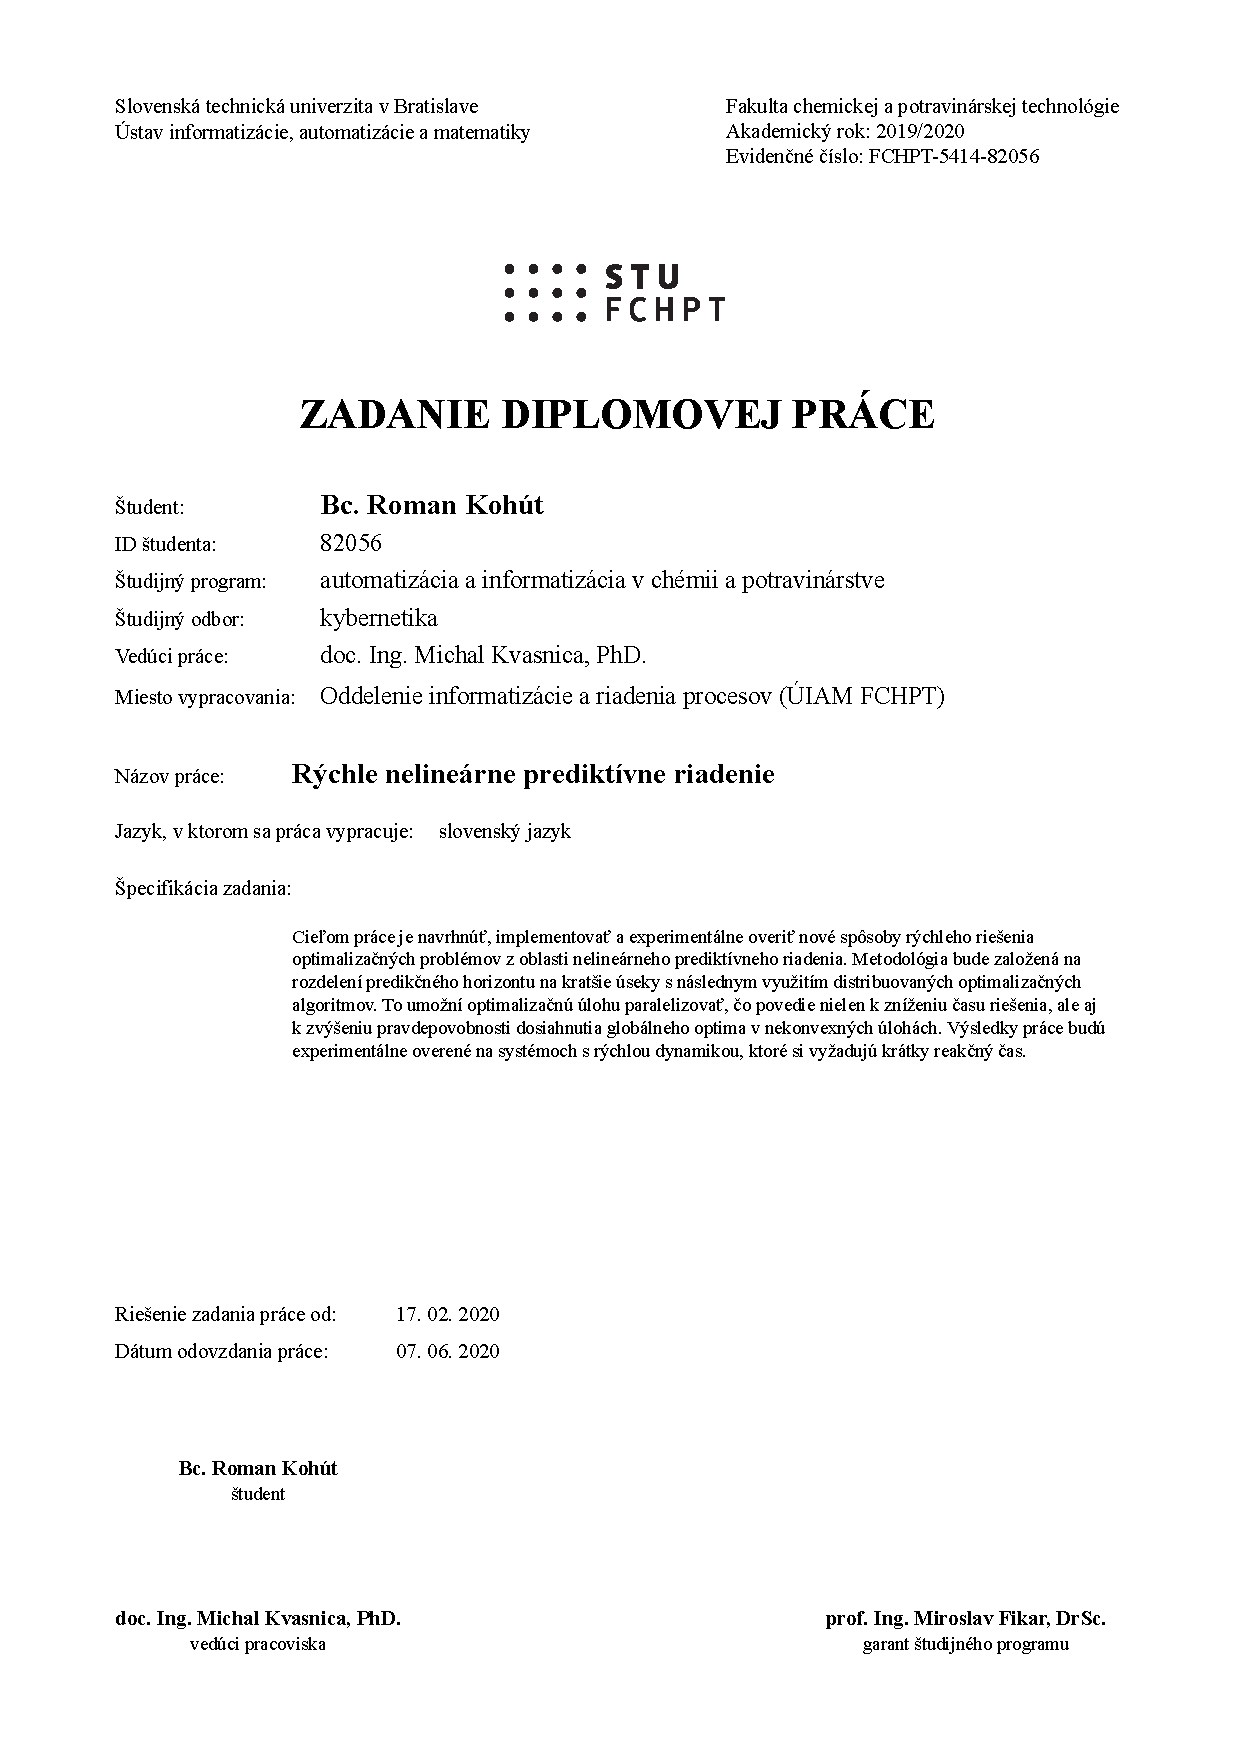
\includepdf[page=1]{content/assignment.pdf}
% use this command only if your assignment has more than 2 pages
% 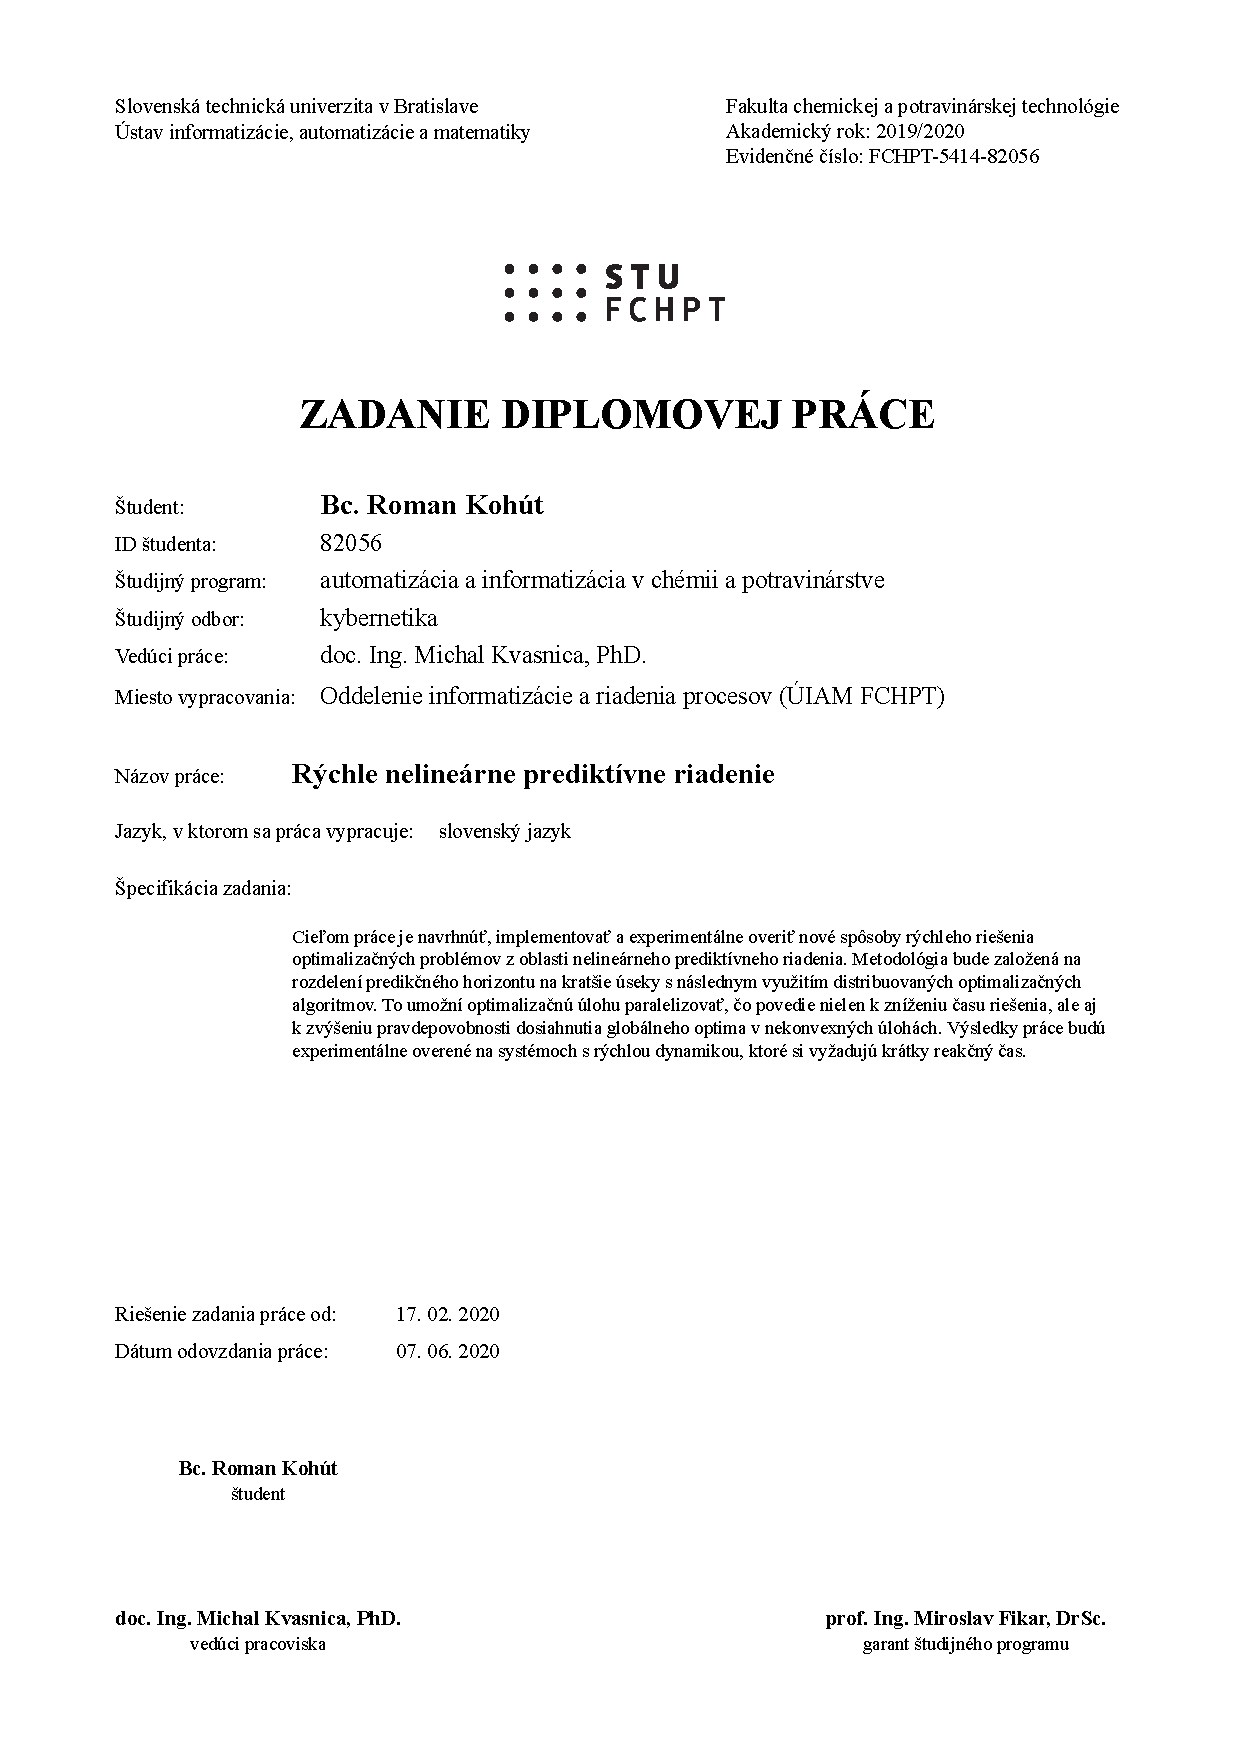
\includepdf[page=2]{content/assignment.pdf}


% do not remove following commands
% do not following commands
\chapter*{\thesisack}
\addcontentsline{toc}{chapter}{\thesisack}
Na tomto mieste by som sa chcel poďakovať môjmu školiteľovi doc. Ing. Michalovi Kvasnicovi, PhD. za užitočné pripomienky, ochotu a usmernenie počas môjho štúdia a pri písaní diplomovej práce.

\chapter*{Abstract}
\markboth{}{}
\addcontentsline{toc}{chapter}{Abstract}
The aim of this master’s thesis is to design and implement a new approach of the fast optimization specifically oriented on the model predictive control. Methodology is based on the distribution of the optimization problem into smaller sections, in model predictive control this means split cost function respect to each step of the prediction horizon. Later we used distributed optimization algorithm with the possibility of a parallel solving and we apply this method on the model predictive control with linear and nonlinear model of the system. In the practical part of this thesis the theory was tested by using simulations in order to determine whether the computational time of the controller will be improved or not. In the last part of this thesis we developed application which allow us to use this kind of model predictive control. The application was divided into two parts. The first one is server which help us to build whole web application. The server is used for data management and for creating a distributed optimization problem. The second part located in the web interface is designed for users whose can use it for defining system and controller parameters. Numerical optimization performed on the background of this interface is used to find minimum of distributed optimization problem. The way  how the application was  designed support parallel solving on multiple computing devices.\\
\textbf{Key words:} model predictive control, distributed optimization algorithm, web application, numerical optimization


\chapter*{Abstrakt}
\markboth{}{}
\addcontentsline{toc}{chapter}{Abstrakt}
Diplomová práca sa venuje návrhu a implementácií nového spôsobu rýchleho riešenia optimalizačných úloh z oblasti prediktívneho riadenia. Metodológia je založená na distribúcií optimalizačnej úlohy na menšie úseky. V prípade prediktívneho regulátora to znamená rozdelenie na jednotlivé kroky predikčného horizontu. Následne sme využili distribuovaný optimalizačný algoritmus s možnosťou paralelného riešenia. Metódu sme aplikovali na prediktívnom riadení s lineárnym aj nelineárnym modelom systému. Praktická časť obsahuje overenie teórie na simuláciách s cieľom zistiť, či takýmto spôsobom vieme zrýchliť výpočtový čas lineárneho aj nelineárneho regulátora. Záver tejto práce je venovaný návrhu aplikácie, pomocou ktorej môžeme využívať daný spôsob riadenia. Aplikáciu sme rozdelili na dve časti. V prvej časti sme vytvorili server, ktorý nám umožňuje vývoj celej webovej aplikácie. Ten tiež slúži na prácu s údajmi a na vytváranie distribuovaného optimalizačného problému. Druhá časť je prístupná používateľom a nachádza sa vo webovom rozhraní. Pomocou nej môže používateľ definovať parametre riadeného systému a prediktívneho regulátora. Na pozadí tohoto rozhrania sa vykonáva numerická optimalizácia, ktorá slúži pre optimalizáciu distribuovaného optimalizačného problému. Takto navrhnutá aplikácia podporuje paralelné riešenie na viacerých výpočtových zariadeniach. \\
\textbf{Kľúčové slová:} prediktívny regulátor, distribuovaný optimalizačný algoritmus, webová aplikácia, numerická optimalizácia

\setcounter{tocdepth}{2}
\renewcommand{\baselinestretch}{0.1}\normalsize
\tableofcontents
\renewcommand{\baselinestretch}{1.5}\large\normalsize
%\renewcommand{\baselinestretch}{1.1}\normalsize

% ----------------------------------------------------------------%
% The Mainmatter !! Do NOT change the structure!!                 %
% ----------------------------------------------------------------%
\mainmatter

% individual chapters should be included via a separate tex file, as shown in 
% here. When working in TexStudio (recomennded tool for Win and Mac) set the 
% main.tex as an Explicit root document, so you can compile even you are
% working on other chapter in other tex file.
%
% Open main.tex THEN click Options-> Root Document -> Set Current Document as
% Explicit Root


\chapter{Úvod}
\label{ch:uvod}

Vo svete málokedy narazíme na také priemyselné odvetvie, v ktorom by sme sa zaobišli bez automatizácie. Či už sa objaví vo forme automatických pohonov alebo jednoduchých logických spínačov automatizácie je a vždy bude súčasťou priemyslu. A zároveň ako je automatizácia neoddeliteľnou súčasťou priemyslu, je aj riadenie procesov súčasťou, bez ktorej by sme sa v automatizácií nezaobišli. Vďaka riadiacim systémom vieme ovládať a ovplyvňovať komplikované procesy ako sú rektifikácie, chemické reaktory, dokonca aj autopilot v aute či lietadle je len bezpečne implementovaný riadiaci systém, ktorý dohliada na hladký chod zariadenia. Kedysi bolo hlavnou úlohou riadiacich systémov dohliadať na správny a bezpečný chod procesu. Avšak s novou dobou sa začalo dostávať do popredia dôležité šetrenie energií, efektivita procesu a mnohé ďalšie. S vývojom technológií a náročnejšími požiadavkami od technológov sa stali riadiace systémy komplikované a jednoduché PID regulátory neboli už schopné zvládať také náročné úlohy. Stalo sa nevyhnutným, aby boli zahrnuté optimalizácie k riadiacim systémom a spresnili tak výpočty. Najčastejšie využívaným riadením s optimalizáciou sa stalo takzvané prediktívne riadenie, založené na modeli, pod skratkou MPC z anglického (Model Predictive Control). Táto metóda zahŕňa matematický model riadeného systému, pomocou ktorého si vieme vypočítať budúce správanie sa procesu niekoľko krokov dopredu (predikčný horizont). Veľkou výhodou takéhoto riadenia sú ohraničenia optimalizácie, v ktorých môžme zahrnúť jednotlivé požiadavky a obmedzenia, dané správaním sa systému. Avšak všetky tieto úlohy musí MPC vedieť riešiť opakovane v malých časových intervaloch a to môže byť problematické. Niekedy je nutné zanedbať isté predpoklady, nájsť vhodnú metódu, riešenie optimalizácie alebo zvoliť malý predikčný horizont, aby sme zrýchlili výpočtový čas MPC a mohli ho tak využiť pre riadenie systému. 

V tejto práci sa budeme venovať implementácií a overeniu novej metódy rýchleho riešenia optimalizačných problémov z oblasti prediktívneho riadenia a cieľom bude znižovanie výpočtového času MPC. Použitá metóda bude založená na rozložení predikčného horizontu na menšie úseky s následným využitím distribuovaného optimalizačného algoritmu. To umožní rozdeliť optimalizačnú úlohu na menšie časti a riešiť ich samostatne, čo povedie k skráteniu času riešenia, ale aj k zvýšeniu pravdepodobnosti dosiahnutia globálneho optima v nekonvexných úlohách.

V teoretickej časti si predstavíme prediktívne riadenie s lineárnym a nelineárnym modelom. V druhej časti teórie si predstavíme optimalizačnú metódu, ktorú využijeme na riešenie a distribuovanie optimalizačného problému. Následne si teóriu overíme na simuláciách v programovacom jazyku Matlab a porovnáme získané údaje s bežne využívaným MPC na systémoch s rýchlou dynamikou. 

Poslednú časť tejto práce venujeme návrhu aplikácie, vďaka ktorej budeme môcť preniesť teóriu do reálneho sveta. Aplikácia bude rozdelená na dve časti častí:
\begin{enumerate}
	\item Serverová časť (Python),
	\item Klientska časť (HTML, CSS, JavaScript).
\end{enumerate}
V programovacom jazyku Python si vytvoríme server, ktorý bude slúžiť na spracovávanie informácií, ich ukladanie a vytváranie optimalizačných úloh. Druhá časť aplikácie bude vo webovom rozhraní, pomocou jazyka HTML, CSS a JavaScript knižnice JQuery si bude môcť klient zadefinovať riadený systém a parametre MPC. A výhradne pomocou jazyka JavaScript sa bude na strane klienta vykonávať numerická optimalizácia. 

Záverom tohoto projektu bude overená teória nového spôsobu rýchleho riešenia optimalizačných problémov z oblasti prediktívneho riadenia na simulácii so systémom s rýchlou dynamikou a aplikácia pomocou, ktorej bude možné využívať takýto spôsob riadenie. 

\chapter{Teória}
\label{part:teoria}

V teoretickej časti si rozoberieme najpoužívanejšie riadenie s optimalizáciou, čo je prediktívne riadenie založené na modeli. Vysvetlíme si spôsob jeho použitia a rozdiel medzi lineárnym a nelineárnym riadením. Druhá polovica teoretickej časti bude venovaná distribuovanému optimalizačnému algoritmu, ktorý bude v práci využívaný a ukážeme, ako môžeme využiť tento algoritmus pri riešení prediktívneho riadenia.

\section{Prediktívne riadenie}
\label{se:teoriaMPC}

Prediktívne riadenie, pod anglickou skratkou MPC, je známe už od minulého storočia. Je jednou z najpoužívanejších foriem riadenia s optimalizáciou. Dokáže zvládať mnohorozmerné riadenie, jedna z jeho najväčších výhod je, že doň vieme zahrnúť ohraničenie. Tým poskytuje obrovskú prevahu oproti svojmu predchodcovi, lineárnemu kvadratickému regulátoru, inak LQR. 

Základnou myšlienkou MPC je, že pomocou známeho matematického modelu systému vieme predikovať budúce správanie sa procesu na pevne určenom časovom horizonte. Tieto informácie vieme využiť pri výpočte optimálnych akčných zásahov, pomocou minimalizácie účelovej funkcie. Takto navrhnuté riadenie nám zabezpečuje garanciu dodržania všetkých ohraničení.

\subsection{Formulácia MPC}
\label{subse:MPC}
Ako sme už spomínali v rámci MPC je nutné poznať matematický model reprezentujúci riadený systém, či už v lineárnej alebo nelineárnej podobe. Najčastejšie sa používa lineárny model v tvare diskrétnej stavovej rovnice v nasledovnej podobe
\begin{align}
	x_{k+1} = Ax_{k} + Bu_{k}\\
	y_{k} = Cx_{k} + Du_{k}
\end{align}
kde $x$ predstavuje stĺpcový vektor stavov o veľkosti $n_{x}$, $u$ predstavuje stĺpcový vektor vstupov o veľkosti $n_{u}$, $A$ je matica stavov definovaná ako $A \in {\rm I\!R}^{n_{x}\times n_{x}}$, B je matica vstupov definovaná ako $B \in {\rm I\!R}^{n_{u}\times n_{u}}$. Rovnicu (2.2), ktorá predstavuje rovnicu výstupu zo systému môžme pri návrhu MPC zanedbať, budeme totiž brať do úvahy iba stavové riadenie.

Základnú formuláciu lineárneho MPC si zadefinujeme nasledovne
\label{math:LinearneMPC}
\begin{subequations}
	\begin{align}
		\displaystyle \min_{u_0,...,u_{N-1}} \hspace{0.1cm} & 
		\sum_{k=1}^{N}\norm{Qx_k}^{2}_{2}+\sum_{k=0}^{N-1}\norm{Ru_k}^{2}_{2}\\
		\textrm{s.t.} \hspace{0.5cm} & x_{k+1} = Ax_{k}+Bu_{k}\hspace{0.5cm} k=0,\dots,N-1\\
		& x_{0} = x(t)\\
		& \underline{x} \leq x_{k} \leq \overline{x}\hspace{0.5cm} k=0,\dots,N\\
		& \underline{u} \leq u_{k} \leq \overline{u}\hspace{0.5cm} k=0,\dots,N-1
	\end{align}
\end{subequations}
kde matica $Q$ predstavuje váhovú maticu stavov definovanú ako $Q \in {\rm I\!R}^{n_{x}\times n_{x}}$, matica $R$ je váhová maticu vstupov definovaná ako $R \in {\rm I\!R}^{n_{u}\times n_{u}}$. Pomocou týchto váhových matíc si môžme nastavovať prioritu počas optimalizácie pre každý stav a vstup samostatne. 

\subsection{Lineárne riadenie s kompenzáciou nelinearity}
\label{subse:LinearneMPCKomp}
Najjednoduchšou formou prediktívneho riadenia je lineárne riadenie. V rámci MPC sa používa lineárny model s lineárnymi ohraničeniami. Ide o najmenej komplikovanú formu, ktorá má výhodu v krátkom výpočtovom čase, čo sa môže hodiť pri systémoch s rýchlou dynamikou. Keďže všetko je vždy o kompromisoch a za rýchlym výpočtovým časom je veľa zanedbaní, ktoré sú najmä v lineárnom modeli. V realite sa málokedy stretneme so systémom, ktorý by stačilo opísať jednoduchým stavovým modelom a riadenie by fungovalo bezchybne. 
\begin{figure}[H]
	\centering
	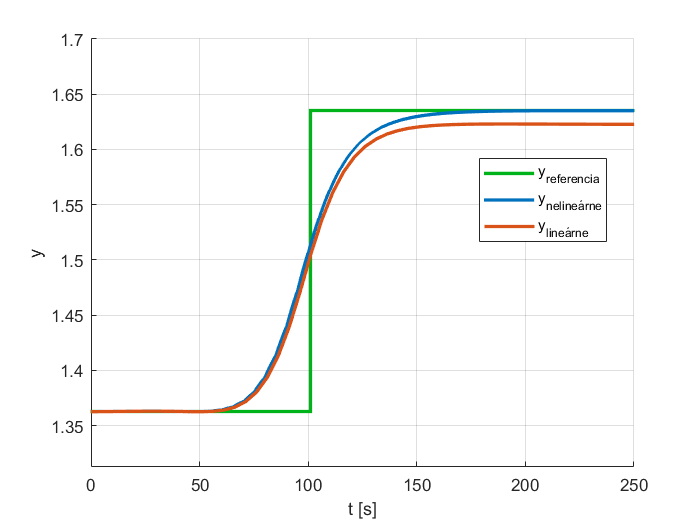
\includegraphics[width=11cm,height=8cm]{images/linear_vs_nonlinear}
	\caption{Rozdiel medzi lineárnim a nelineárnim riadením}
\end{figure}
Pri takomto riadení vznikajú trvalé regulačné odchýlky (Obr.2.1). Aby sa tomu predišlo, musia sa pridávať doplnkové opatrenia, ktoré by vyrovnávali nelinearitu. 

Jedným z najefektívnejších je pridať integračné vlastnosti regulátoru. Pomocou nich bude regulátor minimalizovať rozdiel medzi nelineárnym procesom a lineárnym modelom procesu. Jednoducho sa pridá do lineárneho modelu porucha, ktorá bude reprezentovať tento rozdiel. Takže rovnicu (2.1) nahradíme novým systémom, rozšíreným o poruchu.
\begin{align}
	x_{k+1} &= Ax_{k} + Bu_{k} + Ed_{k}\\
	d_{k+1} &= d_{k}
\end{align}
Nastáva problém, odkiaľ sa získajú aktuálne hodnoty poruchy, reprezentujúcej odchýlku od nelinearity. Takýto člen sa nedá priamo merať senzorom, dá sa ale získať pomocou odhadu. Môžeme využiť buď Luenbergerov pozorovateľ, alebo pokročilejší, časovo premenný Kalmanov filter. 

Výsledná forma takto zadefinovaného MPC bude v nasledovnom tvare.
\begin{subequations}
	\begin{align}
	\displaystyle \min_{u_0,...,u_{N-1}} \hspace{0.1cm} & 
	\sum_{k=1}^{N}\norm{Qx_k}^{2}_{2}+\sum_{k=0}^{N-1}\norm{Ru_k}^{2}_{2}\\
	\textrm{s.t.} \hspace{0.5cm} & x_{k+1} = Ax_{k} + Bu_{k} + E\hat{d}_{k}\hspace{0.5cm} k=0,\dots,N-1\\
	& x_{0} = x(t)\\
	& \hat{d}_{0} = \hat{d}(t)\\
	& \underline{x} \leq x_{k} \leq \overline{x}\hspace{0.5cm} k=0,\dots,N\\
	& \underline{u} \leq u_{k} \leq \overline{u}\hspace{0.5cm} k=0,\dots,N-1
	\end{align}
\end{subequations}
kde $\hat{d}$ predstavuje rozdiel medzi lineárnym a nelineárnym modelom systému, $E$ je jednotková matica definovaná ako $E \in {\rm I\!R}^{n_{x}\times n_{x}}$.

\subsection{Nelineárne riadenie}
\label{subse:NelinearneMPC}
Ak by sme chceli predísť všetkým prídavkom k lineárnemu riadeniu a následnému ladeniu všetkých pridaných váhových matíc, je možnosť priamo vymeniť lineárny model za nelineárny. V rámci tejto práce sa budeme venovať práve takémuto nelineárnemu riadeniu, tak, že nahradíme lineárny model používaný v MPC priamo za nelineárny.

Nelineárne rovnice budú vo forme diferenciálnych rovníc, ktoré následne diskretizujeme v rámci periódy vzorkovania systému. Takto získanú rovnicu použijeme miesto stavového opisu a výsledné MPC bude mať nasledovnú formu.
\begin{subequations}
	\begin{align}
	\displaystyle \min_{u_0,...,u_{N-1}} \hspace{0.1cm} & 
	\sum_{k=1}^{N}\norm{Qx_k}^{2}_{2}+\sum_{k=0}^{N-1}\norm{Ru_k}^{2}_{2}\\
	\textrm{s.t.} \hspace{0.5cm} & x_{k+1} = f(x_{k},u_{k},T_{s})\hspace{0.5cm} k=0,\dots,N-1\\
	& x_{0} = x(t)\\
	& \underline{x} \leq x_{k} \leq \overline{x}\hspace{0.5cm} k=0,\dots,N\\
	& \underline{u} \leq u_{k} \leq \overline{u}\hspace{0.5cm} k=0,\dots,N-1
	\end{align}
\end{subequations}
Takýto prístup môže spôsobiť komplikácie pri riešení MPC. Výrazne sa zväčší výpočtový čas a je komplikovanejšie s ním narábať. Cieľom tejto práce bude zrýchliť aj takéto riadenie tak, aby ho bolo možné využiť pri systémoch s rýchlou dynamikou.


\section{Eulerova metóda diskretizácie}
\label{se:diskretizacia}
Táto metóda je stará už vyše 200 rokov, ale aj napriek tomu sa používa dodnes. Je založená na numerickej diskretizácii. Chyba, ktorej sa dopúšťame použitím tejto metódy, je priamo úmerná kroku diskretizácie, ktorý zvolíme. Nie je až taká účinná v porovnaní s ostatnými metódami, ale je používaná ako základ komplexnejších metód. Pre účely nášho projektu bude postačujúca v základnej forme a jej jednoduchosť bude pre nás výhodou.

Majme nasledovnú vzťah:
\begin{align}
		\dot{x}(t) &= f(x,t),
\end{align}
kde $\dot{x}(t)$ predstavuje diferenciálnu rovnicu $\dot{x}(t)=\frac{dx(t)}{dt}$, ktorá opisuje modle systému v kontinuálnom čase. Pomocou Eulerovej metódy ju môžeme nasledovne pretransformovať:
\begin{align}
	x_{k+1} &= x_{k} + hf(x_{k}),
\end{align}
kde h predstavuje dĺžku kroku, v našom projekte bude rovnaká, ako perióda vzorkovania diskretizovaného systému.
\begin{figure}[H]
	\centering
	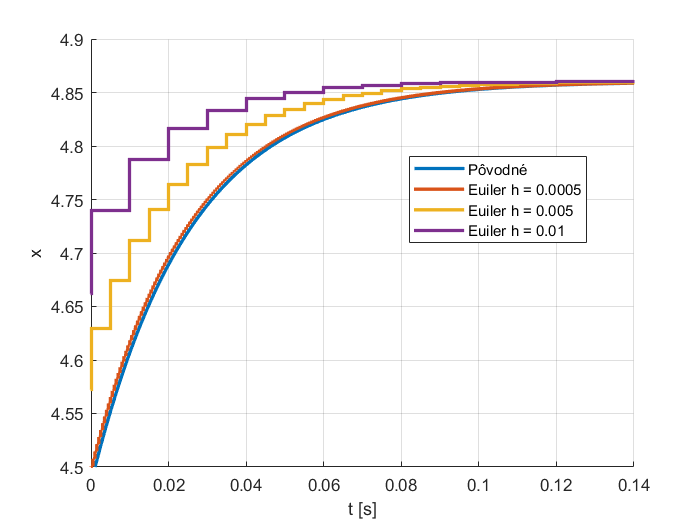
\includegraphics[width=11cm,height=8cm]{images/Euler_method}
	\caption{Eulerová diskretizácia}
\end{figure}
Ako môžeme vidieť na (Obr. 2.1), čím budeme používať menšiu periódu, tým presnejšia bude diskretizácia.


\section{Decentralizovaná optimalizácia}
\label{se:DecentralizovanaOptimalizacia}
Zvyčajne, pri všeobecnej optimalizačnej úlohe, si ako prvé zadefinujeme účelovú funkciu, určíme si začiatočné podmienky a ohraničenia potom zvolíme vhodnú optimalizačnú metódu pre nájdenie optima. Takto formulovanú optimalizáciu nazývame centralizovaná optimalizácia, kde sa všetky premenné nachádzajú pod jedným problémom a výsledkom je centralizované riešenie. 
\begin{subequations}
	\begin{align}
		\displaystyle \min_{x} \hspace{0.5cm} & 
		f(x)\\
		\textrm{s.t.} \hspace{0.5cm} & Lx = v
	\end{align}
\end{subequations}
V tejto práci ale využijeme takzvanú decentralizáciu optimalizačného problému. Optimalizačnú úlohu si rozložíme na viacero častí $ f(x) = g(z) + h(y)$ a každú riešime samostatne. Výsledkom bude viacero decentralizovaných riešení.
\begin{subequations}
	\begin{align}
		\displaystyle \min_{} \hspace{0.5cm} & 
		g(z) + h(y)\\
		\textrm{s.t.} \hspace{0.5cm} & L_{1}z = v_1\\
		& L_{2}y = v_2
	\end{align}
\end{subequations}
Takéto rozloženie účelovej funkcie na viac častí umožňuje zjednodušenie optimalizačnej úlohy a pri riešení náročných optimalizácií môže výrazne skrátiť čas výpočtu.
\begin{figure}[H]
	\centering
	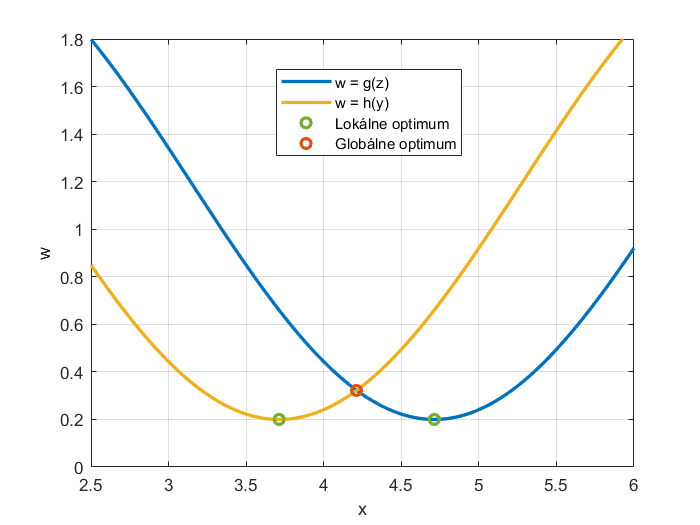
\includegraphics[width=11cm,height=8cm]{images/Global_Local_ADM}
	\caption{Porovnanie globálneho a lokálneho riešenia}
\end{figure}
Jedným z problémov, ktorý môže nastať pri decentralizovanej optimalizácií je, že jednotlivé decentrálne riešenia môžu uviaznuť vo svojich lokálnych optimách (Obr. 2.3). Cieľom decentralizovanej optimalizácie bude aj, aby jednotlivé riešenia nekonvergovali do lokálneho, ale do jedného globálneho. 
\subsection{ADMM}
\label{subse:ADMM}
ADMM je skratka z anglického názvu (Alternating Direction Method of Multipliers). Pomocou tejto metódy vieme riešiť decentralizovaný optimalizačný problém.
Formulácia optimalizačného problému pre ADMM je v nasledovnom tvare
\begin{subequations}
	\begin{align}
		\displaystyle \min_{y,z} \hspace{0.5cm} & 
		g(z) + h(y),\\
		\textrm{s.t.} \hspace{0.5cm} & H_{1}z + H_{2}y = b,
	\end{align}
\end{subequations}
kde $y$ a $z$ sú optimalizované premenné, ktoré sú definované nasledovne $y \in {\rm I\!R}^n $, $ z\in {\rm I\!R}^m$. Rovnica (2.12b) predstavuje novú podmienku, ktorá prepája decentralizované premenné, matica $H_{1}$, $H_{2}$ a vektor $b$ sú skonštruované tak, aby podmienky boli vhodné pre všetky prípady, ich rozmery sú $H_{1} \in {\rm I\!R}^{p \times n}$, $H_{2} \in {\rm I\!R}^{p \times m}$ a teda vo výsledku je vektor $b \in {\rm I\!R}^p $. 

Ako môžeme vidieť, rozdiel medzi decentralizovaným a centralizovaným optimalizačným problémom je, že sme rozdelili optimalizované premenné, spolu s účelovou funkciou, ktorá musí umožňovať takéto rozdelenie premenných. S takýmto rozdelením nám zároveň pribudla nová podmienka do optimalizačného problému, ktorá prepája rozdelenú funkciu. Táto podmienka sa nazýva duálna funkcia. 
Ďalej môžeme pokračovať tak, že túto novú podmienku pridáme do optimalizačného problému pomocou Lagrangeovej metódy a vytvoríme rozšírený lagrangeán.
\begin{equation}
	\mathcal{L}_{\rho} = g(z) + h(y) + \lambda^{T}\left(  H_{1}z + H_{2}y - b \right) + \frac{\rho}{2} \norm{H_{1}z + H_{2}y - b}_{2}^{2}
\end{equation}
Rozšírenie lagrangeánu predstavuje posledný člen $\frac{\rho}{2} \norm{H_{1}z + H_{2}y - b}_{2}^{2}$ a zabezpečuje, aby bola funkcia spojite diferencovateľná a zároveň pomáha konvergencii. Pridaním tohoto člen neovplyvníme hodnotu optima, keďže je v optime nulové. Takto definovanú úlohu vieme riešiť separátnym prístupom k jednotlivým premenným lagrangianu $\mathcal{L}_{\rho} \left(z,y,\lambda \right)$
\label{math:ADMM_iteracie}
\begin{align}
	&z^{(i+1)} = \argmin_{z} \mathcal{L}_{\rho} \left(z,y^{i},\lambda^{i} \right),\\
	&y^{(i+1)} = \argmin_{y} \mathcal{L}_{\rho} \left(z^{i},y,\lambda^{i} \right),\\
	&\lambda^{(i+1)} = \lambda^{i} + \rho( H_{1}z^{(i+1)} + H_{2}y^{(i+1)} - b ),
\end{align}
kde $\rho > 1$. Táto iteračná metóda prebieha v takzvanom duálnom framworku, ktorý sa skladá z primárneho problému (minimalizácia $z$, minimalizácie $y$) a aktualizácie duálneho problému $\lambda$. V poslednom vzťahu, kde sa aktualizuje duálna premenná, je aplikovaný podobný postup ako v numerickej gradientovej metóde, ale vykoná sa iba raz, $\rho$ tu predstavuje dĺžku kroku. Funkcia tohoto duálneho problému je konkávna, a teda sa ľahko maximalizuje, čo nespôsobuje ťažkosti, ak náš primárny problém je konvexný. Ak primárny problém spĺňa konvexnosť tak jeho minimum korešponduje s maximom duálneho problému. Preto neoptimalizujeme v smere poklesu (ako tomu je pri minimalizácii v gradientovej metóde), ale hýbeme sa v smere rastu\cite{bib1}. 
\label{subse:ADMM2}

Postup pri iterácií v ADMM.
\begin{description}
	\item[Krok 1:] {Paralelne vyriešime minimalizáciu lagrangeana vzhľadom k všetkým predikčným horizontom, \hyperref[math:ADMM_iteracie]{rovnice (2.14,2.15)}.}
	\item[Krok 2:] {Aktualizujeme duálny parameter $\lambda$ s novými hodnotami, \hyperref[math:ADMM_iteracie]{rovnica (2.16)}.}
	\item[Krok 3:] {Opakujeme od kroku 1, až kým skonvergujeme do globálneho minima (narazíme na zastavovacie kritérium).}
\end{description}



\section{Prediktívne riadenie pomocou ADMM}
\label{se:MPC_ADMM}
V tejto časti teórie spojíme \hyperref[subse:MPC]{MPC(2.1.1)} a \hyperref[subse:ADMM]{ADMM (2.4)}. Najskôr aplikujeme ADMM na lineárnom riadení, ukážeme si ako rozložiť MPC podla predikčných horizontov a vysvetlíme si spôsob, akým budeme získavať optimálne decentralizované riešenia. V druhej časti si ukážeme, čo všetko musíme nahradiť a upraviť, aby sme boli schopní použiť ADMM pri nelineárnom riadení. 

\subsection{Linearne prediktívne riadenie}
\label{subse:Lin_MPC_ADMM}
Ako sme už spomínali, v tejto časti využijeme ADMM pre lineárne riadenie. Takže naším cieľom bude overiť funkčnosť paralelného riešenia decentralizovaného optimalizačného problému so snahou zrýchliť výpočet MPC. Myšlienka spočíva v rozdelení MPC na $N$ predikčných horizontov a následné paralelné riešenie decentralizovaného MPC. Tento výpočet bude prebiehať na viacerých počítačoch, ktoré budú hľadať centralizované riešenie. 

Majme linearne MPC bez ohraničení:
\label{math:2.14}
\begin{subequations}
	\begin{align}
		\displaystyle \min_{u_0,...,u_{N-1}} \hspace{0.1cm} & 
		\sum_{k=1}^{N}\norm{Qx_k}^{2}_{2}+\sum_{k=0}^{N-1}\norm{Ru_k}^{2}_{2},\\
		\textrm{s.t.} \hspace{0.5cm} & x_{k+1} = Ax_{k}+Bu_{k}\hspace{0.5cm} k=0,\dots,N-1,\\
		& x_{0} = x(t).
	\end{align}
\end{subequations}
Postupujeme podla teórie uvedenej v \hyperref[subse:ADMM]{(2.4)}. Takto formulované MPC si môžeme rozdeliť na $2,\dots,N$ decentralizovaných problémov. Budeme pracovať s úplnou decentralizáciou a MPC si rozdelíme na $N$ decentralizovaných optimalizačných problémov.
\label{math:ADMM_MPC}
Ako príklad si zoberme MPC pre predikčný horizont $N = 3$:
\begin{subequations}
	\begin{align}
		\displaystyle\min_{u_0,u_1,u_2}\hspace{0.1cm}&\norm{Qx_1}^{2}_{2}+\norm{Qx_2}^{2}_{2}+\norm{Qx_3}^{2}_{2}+\norm{Ru_0}^{2}_{2}+\norm{Ru_1}^{2}_{2}+\norm{Ru_2}^{2}_{2},\\
		& x_{0} = x(t),\\
		&x_{1} = Ax_{0}+Bu_{0},\\
		&x_{2} = Ax_{1}+Bu_{1},\\
		&x_{3} = Ax_{2}+Bu_{2}.
	\end{align}
\end{subequations}
Za každý stav si môžeme dosadiť model systému v príslušnom kroku $k=1,\dots,3$:
\begin{subequations}
	\begin{align}	
	\begin{split}			
			\displaystyle\min_{u_0,u_1,u_2}\hspace{0.1cm}&\norm{Q(Ax_{0}+Bu_{0})}^{2}_{2}+\norm{Ru_0}^{2}_{2}+\norm{Q(Ax_{1}+Bu_{1})}^{2}_{2}+\norm{Ru_1}^{2}_{2}+\\
			&\norm{Q(Ax_{2}+Bu_{2})}^{2}_{2}+\norm{Ru_2}^{2}_{2}
	\end{split}\\
	& x_{0} = x(t).
	\end{align}
\end{subequations}
Teraz máme optimalizačný problém, ktorý chceme optimalizovať pre každý predikčný horizont samostatne. Takže pre každý stav musíme poznať počiatočné podmienky ($x_0,x_1,x_2$). V našom prípade máme počiatočné podmienky iba pre prvý stav, rovnica (2.16b), čiže ostatné musíme hľadať. Práve k tomu nám dopomôže duálna funkcia, ktorá bude koordinovať hľadané počiatočné stavy s ich skutočnými hodnotami. 

Duálna funkcia bude vychádzať z modelu systému \hyperref[math:2.14]{(2.14b)} a prepíšeme si ju do nasledovnej podoby:
\begin{align}
	H_{1}u_{k-1} + H_{2}x_{k} = -Ax_{k-1},
\end{align}
kde $H_{1} = B$ a je definované ako $H_{1} \in {\rm I\!R}^{n_{u}\times n_{u}}$, $H_{2}$ je záporná jednotková matica definovaná ako $H_{2} \in {\rm I\!R}^{n_{x}\times n_{x}}$. Pridáme túto duálnu funkciu do nášho všeobecného optimalizačného problému:
\begin{subequations}
	\begin{align}
		\displaystyle \min_{u_0,...,u_{N-1},x_1,...,x_N} \hspace{0.1cm} & 
		\sum_{k=1}^{N}
		\norm{Qx_k}^{2}_{2}+\sum_{k=0}^{N-1}\norm{Ru_k}^{2}_{2},\\
		\textrm{s.t.} \hspace{1.1cm} & x_{n+1} = Ax_{k}+Bu_{k} \hspace{0.5cm} k=0,\dots,N-1,\\
		& x_{0} = x(t),\\
		&H_{1}u_{k-1} + H_{2}x_{k} = -Ax_{k-1}\hspace{0.5cm} k=1,\dots,N.
	\end{align}
\end{subequations}
Pomocou upravenej Lagrangianovej metódy sa zbavíme duálnej funkcie (2.21d) a vytvoríme rozšírenú Lagrangianovú funkciu:
\label{math:RozsirenyLag}
\begin{equation}
\begin{split}
\mathcal{L}_{\rho} =&~ \sum_{k=0}^{N-1}\norm{Q(Ax_{k}+Bu_{k})}^{2}_{2}+\sum_{k=0}^{N-1}\norm{Ru_k}^{2}_{2} +\\+&~\sum_{k=1}^{N-1}\lambda_{k}^{T}\left(  H_{1}u_{k-1} + H_{2}x_{k} + Ax_{k-1}\right) +\\+&~\sum_{k=1}^{N-1}\frac{\rho}{2} \norm{H_{1}u_{k-1} + H_{2}x_{k} + Ax_{k-1}}_{2}^{2}
\end{split}
\end{equation}
Pre zjednodušenie využijeme substitúciu pre jednotlivé premenné našej optimalizácie:
\begin{align}
	U_{0} =\begin{bmatrix}
	u_{0}\\
	x_{0}
	\end{bmatrix},
	U_{1} =\begin{bmatrix}
	u_{1}\\
	x_{1}
	\end{bmatrix}, \dots ,
	U_{k} =\begin{bmatrix}
	u_{k}\\
	x_{k}
	\end{bmatrix}.
\end{align}
Dosadíme jednotlivé substituované premenné do rovnice \hyperref[math:RozsirenyLag]{(2.19)}, rozšírime si matice vzhľadom k substituovaným premenným a dostaneme nasledovný vzťah:
\label{math:RozsirenyLag2}
\begin{equation}
\begin{split}
\mathcal{L}_{\rho} =&~ \sum_{k=0}^{N-1}\norm{\tilde{Q}(\tilde{A}U_{k}+\tilde{B}U_{k})}^{2}_{2}+\sum_{k=0}^{N-1}\norm{\tilde{R}U_k}^{2}_{2} +\\&~\sum_{k=1}^{N-1}\lambda_{k}^{T}\left(  \tilde{H}_{1}U_{k-1} + \tilde{H}_{2}U_{k} + \tilde{A}U_{k-1} \right) +\\&~\sum_{k=1}^{N-1}\frac{\rho}{2} \norm{\tilde{H}_{1}U_{k-1} + \tilde{H}_{2}U_{k} + \tilde{A}U_{k-1}}_{2}^{2}
\end{split}
\end{equation}
kde $U$ je definované ako $U \in {\rm I\!R}^{p\times1}, p = n_{x} + n_{u}$, počet rovníc je $r$, potom všetky rozšírené matice sú definované ako $(\tilde{A}$, $\tilde{B}$, $\tilde{Q}$, $\tilde{R}$, $\tilde{H}_{1}$, $\tilde{H}_{2}) \in {\rm I\!R}^{r \times p}$.
 Jednotlivé rozšírené matice sú zložené nasledovne:
\begin{subequations}
	\begin{align}
		&\tilde{A} = \begin{bmatrix}
						0\\
						A
					\end{bmatrix},\\
		&\tilde{B} = \begin{bmatrix}
							B & 0
					 \end{bmatrix},\\
		&\tilde{Q} = \begin{bmatrix}
						0 & Q
					 \end{bmatrix},\\
		&\tilde{R} = \begin{bmatrix}
						R & 0
					\end{bmatrix},\\
		&\tilde{H}_{1} = \begin{bmatrix}
							B & 0
						\end{bmatrix},\\
		&\tilde{H}_{2} = \begin{bmatrix}
							0 & -I
						\end{bmatrix}.
	\end{align}
\end{subequations}
\label{math:Linear_Lagrangean}\noindent
Ako môžeme vidieť, takto upravenú Lagrangianovú funkciu môžeme jednoducho optimalizovať vzhľadom k jednotlivým krokom predikčného horizontu:
\begin{subequations}
	\begin{align}
	&u_{0}^{(i+1)} = \argmin_{u_{0}} \mathcal{L}_{\rho} \left(u_{0},x_{0},x_{1}^{i},\lambda_{1}^{i}\right)\\
	&U_{k}^{(i+1)} = \argmin_{U_{k}} \mathcal{L}_{\rho} \left(U_{k},U_{k-1}^{i},\lambda_{k}^{i},U_{k+1}^{i},\lambda_{k+1}^{i}\right) \hspace{0.5cm} k=1,\dots,N-2\\
	&U_{k}^{(i+1)} = \argmin_{U_{k}} \mathcal{L}_{\rho}\left(U_{k},U_{k-1}^{i},\lambda_{k}^{i}\right) \hspace{0.5cm} k=N-1\\
	&\lambda_{k}^{(i+1)} = \lambda_{k}^{i} + \rho( \tilde{H}_{1}U_{k-1}^{(i+1)} + \tilde{H}_{2}U_{k}^{(i+1)} - \tilde{A}U_{k-1})\hspace{0.5cm} k=1,\dots,N-1
	\end{align}
\end{subequations}
Postup pri iterácií v ADMM sme si vysvetlili v kapitole \hyperref[subse:ADMM2]{(2.4)}. Keďže pracujeme s lineárnym modelom, pre minimalizáciu Lagrangianovej funkcie sme si zvolili analytickú metódu optimalizácie. Nájdeme teda gradient Lagrangianovej funkcie vzhľadom k optimalizovanej premennej, položíme ho rovný nule a vyjmeme si optimalizovanú premennú:
\begin{align}
&\frac{\partial \mathcal{L}_{\rho}}{\partial U_{k}} = 0  \hspace{0.5cm} \Longrightarrow  \hspace{0.5cm} U_{k}^{*}.
\end{align}
Vzhľadom na to, že používame analytické riešenie optimalizácie, môžeme nájsť všeobecné vzťahy, ktoré budú vždy platné.
Máme tri prípady, ktoré môžu nastať \hyperref[math:Linear_Lagrangean]{rovnice (2.31a,2.31b,2.31c)}
\begin{enumerate}
	\item{Prvý krok predikčného horizontu $k = 0$, v tomto prípade musíme urobiť výnimku, keďže derivácia podla konštanty $x_0$ je nulová, teda nemôžme použiť rozšírenú formu Lagrangianovej funkcie \hyperref[math:RozsirenyLag]{(2.21)}, ale využijeme jej základnú formu  \hyperref[math:RozsirenyLag]{(2.19)}:\\
		\begin{subequations}
			\begin{align}
				\begin{split}
					&\mathcal{L}_{\rho} =\norm{Q(Ax_{0}+Bu_{0})}^{2}_{2}+\norm{Ru_{0}}^{2}_{2} +\lambda_{1}^{T}\left(H_{1}u_{0} + H_{2}x_{1} + Ax_{0} \right)+\\&\hspace{0.8cm}\norm{H_{1}u_{0} + H_{2}x_{1} + Ax_{0}}_{2}^{2}+\dots
				\end{split}\\
				&\frac{\partial \mathcal{L}_{\rho}\left(u_{0},x_{0},x_{1}^{i},\lambda_{1}^{i}\right)}{\partial u_{0}} = 0,\\
				&u_{0}^{*} = -M_{0}^{-1}\left(2B^{T}Q^{T}QAx_{0}+H_{1}^{T}(\lambda_{1}^{i}+\rho H_{2}x_{1}^{i}+\rho Ax_{0})\right),\\
				&M_{0} = 2B^{T}Q^{T}QB + 2R^{T}R +\rho H_{1}^{T}H_{1}.
			\end{align}
		\end{subequations}
	}
	\item{Keď krok predikčného horizontu $k$ sa nachádza v otvorenom intervale $\left(0,N-1\right)$:\\
		\begin{subequations}
			\begin{align}
				&\frac{\partial \mathcal{L}_{\rho}\left(U_{k},U_{k-1}^{i},\lambda_{k}^{i},U_{k+1}^{i},\lambda_{k+1}^{i}\right)}{\partial U_{k}} = 0,\\
				&U_{k}^{*} = -M_{n}^{-1}\left(\tilde{H}_{2}^{T}f_{1}(\lambda_{k}^{i},U_{k-1}^{i})+(\tilde{H}_{1}^{T}+\tilde{A}^{T})f_{2}(\lambda_{k+1}^{i},U_{k+1}^{i})\right),\\
				\begin{split}
					& M_{n} = 2\tilde{A}^{T}\tilde{Q}^{T}\tilde{Q}\tilde{A}+2\tilde{A}^{T}\tilde{Q}^{T}\tilde{Q}\tilde{B}+2\tilde{B}^{T}\tilde{Q}^{T}\tilde{Q}\tilde{B}+2\tilde{B}^{T}\tilde{Q}^{T}\tilde{Q}\tilde{A}+\\
					&\hspace{1.0cm}2\tilde{R}^{T}\tilde{R} + \rho\tilde{H}_{2}^{T}\tilde{H}_{2}+ \rho\tilde{H}_{1}^{T}\tilde{H}_{1} + \rho\tilde{H}_{1}^{T}\tilde{A} + \rho\tilde{A}^{T}\tilde{H}_{1}+ \rho\tilde{A}^{T}\tilde{A}
				\end{split}\\
				& f_{1}(\lambda_{k}^{i},U_{k-1}^{i}) = \lambda_{k}^{i} + \rho\tilde{H}_{1}U_{k-1}^{i}+\rho\tilde{A}U_{k-1}^{i},\\
				& f_{2}(\lambda_{k+1}^{i},U_{k+1}^{i}) = \lambda_{k+1}^{i} + \rho\tilde{H}_{2}U_{k+1}^{i}.
			\end{align}
		\end{subequations}
	}
		\item{Posledný krok predikčného horizontu $k = N-1$:\\
		\begin{subequations}
			\begin{align}
			&\frac{\partial \mathcal{L}_{\rho}\left(U_{k},U_{k-1}^{i},\lambda_{k}^{i}\right)}{\partial U_{k}} = 0,\\
			&U_{k}^{*} = -M_{N}^{-1}\tilde{H}_{2}^{T}f_{1}(\lambda_{k}^{i},U_{k-1}^{i}),\\
			\begin{split}
			& M_{N} = 2\tilde{A}^{T}\tilde{Q}^{T}\tilde{Q}\tilde{A}+2\tilde{A}^{T}\tilde{Q}^{T}\tilde{Q}\tilde{B}+2\tilde{B}^{T}\tilde{Q}^{T}\tilde{Q}\tilde{B}+2\tilde{B}^{T}\tilde{Q}^{T}\hat{Q}\tilde{A}+\\
			&\hspace{1.0cm}2\tilde{R}^{T}\tilde{R} + \rho\tilde{H}_{2}^{T}\tilde{H}_{2}
			\end{split}\\
			& f_{1}(\lambda_{k}^{i},U_{k-1}^{i}) = \lambda_{k}^{i} + \rho\tilde{H}_{1}U_{k-1}^{i}+\rho\tilde{A}U_{k-1}^{i}.
			\end{align}
		\end{subequations}
	}
\end{enumerate}
Kde $u_{0}^{*}$ a $U_{k}^{*}$ predstavuje naše rovnice pre získanie optimálnych hodnôt akčných zásahov a počiatočných stavov. Takto zadefinované rovnice môžeme rovno používať v ADMM.

\subsection{Nelinearne prediktívne riadenie}
\label{subse:Nelin_MPC_ADMM}
V tejto časti sa budeme venovať nelineárnemu riadeniu. Na rozdiel od lineárneho MPC, implementácia algoritmu je omnoho komplikovanejšia. Pretože musí zvládať rýchle on-line riešenie. Práve pri takejto komplikovanej optimalizačnej úlohe nám môže pomôcť ADMM.

Nelinearita optimalizačnej úlohy sa môže prejavovať vo viacerých formách, napríklad nelineárna účelová funkcia, nelineárny model systému alebo nelineárne ohraničenia. My sme sa zamerali konkrétne na nelineárny model. 
Zadefinujeme si MPC v nasledovnom tvare:
\begin{subequations}
	\begin{align}
	\displaystyle \min_{u_0,...,u_{N-1}} \hspace{0.1cm} &\sum_{k=1}^{N}\norm{Qx_k}^{2}_{2}+\sum_{k=0}^{N-1}\norm{Ru_k}^{2}_{2},\\
	\textrm{s.t.} \hspace{0.5cm} & x_{k+1} = f(x_{k},u_{k})\hspace{0.5cm} k=0,\dots,N-1,\\
	& x_{0} = x(t).
	\end{align}
\end{subequations}
Rovnako ako pri lineárnom MPC v časti \hyperref[math:ADMM_MPC]{(2.5.1)} si rozdelíme optimalizačnú úlohu na $N$ decentralizovaných problémov a následne si zadefinujeme duálne funkcie:
\begin{subequations}
	\begin{align}
	\displaystyle \min_{u_0,...,u_{N-1},x_1,...,x_N}\hspace{0.1cm} & 
	\sum_{k=1}^{N}
	\norm{
		Qx_k
	}^{2}_{2}
	+
	\sum_{k=0}^{N-1}\norm{
		Ru_k
	}^{2}_{2},\\
	\textrm{s.t.} \hspace{1.1cm} & x_{k+1} = f(x_{k},u_{k})\hspace{0.5cm} k=0,\dots,N-1,\\
	& x_{0} = x(t),\\
	& x_{k}(x_{k-1},u_{k-1})- x_{k} = 0 \hspace{0.5cm} k=1,\dots,N-1.
	\end{align}
\end{subequations}
Na rozdiel od lineárneho MPC sú tieto podmienky, rovnako ako aj model, nelineárne. Čiže sú, z výpočtového hľadiska, náročnejšie na získanie. Ako v predošlých postupoch vytvorime si rozšírenú Lagrangianovú funkciu:
\begin{equation}
\begin{split}
\mathcal{L}_{\rho} =&~ \sum_{k=0}^{N-1}
\norm{
	Qf(x_{k},u_{k})
}^{2}_{2}
+
\sum_{k=0}^{N-1}\norm{
	Ru_k
}^{2}_{2}+\\+&~\sum_{k=1}^{N-1}\lambda_{k}^{T}\left( x_{k}(x_{k-1},u_{k-1}) - x_{k} \right) +\\+&~\sum_{k=1}^{N-1}\frac{\rho}{2} \norm{ x_{k}(x_{k-1},u_{k-1}) - x_{k}}_{2}^{2}
\end{split}
\end{equation}
ktorú budeme riešiť separátne vzhľadom k jednotlivým krokom predikčného horizontu:
\begin{subequations}
\begin{align}
	&u_{0}^{(i+1)} = \argmin_{u_{0}} \mathcal{L}_{\rho} \left(u_0,x_{0},u_1^{i},x_{1}^{i},\lambda_{1}^{i}\right),\\
	\begin{split}
		&\begin{bmatrix}
		u_{k}^{(i+1)} \\
		x_{k}^{(i+1)}
		\end{bmatrix} = 
		\argmin_{u_{k},x_{k}} \mathcal{L}_{\rho} (u_{k},x_{k},u_{k-1}^{i},x_{k-1}^{i},\lambda_{k}^{i},\\
		&\hspace{3.5cm}u_{k+1}^{i},x_{k+1}^{i},\lambda_{k+1}^{i})\hspace{0.5cm} k=1,\dots,N-2
	\end{split}\\
	&\begin{bmatrix}
		u_{k}^{(i+1)} \\
		x_{k}^{(i+1)}
	\end{bmatrix} = \argmin_{u_{k},x_{k}} \mathcal{L}_{\rho} \left(u_{k},x_{k},u_{k-1}^{i},x_{k-1}^{i},\lambda_{k-1}^{i}\right) \hspace{0.5cm} k=N-1,\\
	&\lambda_{k}^{(i+1)} = \lambda_{k}^{i} + \rho( x_{k}(x_{k-1}^{(i+1)},u_{k-1}^{(i+1)}) - x_{k}^{(i+1)}) \hspace{0.5cm} k=1,\dots,N-1.
\end{align}
\end{subequations}
Zmena nastáva vo forme riešenia týchto optimalizačných problémov. 
Nelineárne modely bývajú často komplikované. Ich dosadenie do účelovej funkcie, vytvorenie analytického gradientu a vyjadrenie neznámych môže byť zložitejšie, než sa na prvý pohlaď zdá. Často tieto analytické vyjadrenia bývajú tak pamäťovo náročné, že je omnoho ľahšie siahnuť po numerickej optimalizácií. A tak sme aj my v tejto práci využili numerickú optimalizáciu, konkrétne Newtonowu metódu. 

\label{opt:Newton}
Newtonova numerická optimalizácia je vylepšená Gradientová metóda, ktorá je založená nielen na gradiente, ale aj Hessovej matici optimalizovanej funkcie. Môžeme si túto metódu zadefinovať nasledovne:
\begin{subequations}
\begin{align}
&\Delta x = -\nabla^{2}f(x)^{-1} \nabla f(x), \\
& x^{*} = x + \Delta x,
\end{align}
\end{subequations}
kde $\Delta x$ predstavuje smer poklesu funkcie (keďže ide o minimalizáciu), $\nabla^{2}f(x)$ je Hessova matica a $\nabla f(x)$ je gradient funkcie, konštanta $t$ určuje veľkosť kroku. 
Túto veľkosť kroku nebudeme mať statickú, ale využijeme takzvaný backtracking, ktorý bude meniť $t$ s každou iteráciou v optimalizácii.

Postup pri iteráciách v Newtonovej metóde je nasledovný.
\begin{description}
	\item[Krok 1:] {Zvolíme si začiatočný bod $x$.}
	\item[Krok 2:] {Zavoláme gradient funkcie $\nabla f(x^{i})$ a Hessovu maticu $\nabla^{2} f(x^{i})$.}
	\item[Krok 3:] {Vypočítame smer poklesu $\Delta x = -\nabla^{2}f(x^{i})^{-1} \nabla f(x^{i})$.}
	\item[Krok 4:] {Pomocou backtrackingu nájdeme vhodný krok $t$ a aktualizujeme optimalizované premenné $x^{i+1} = x^{i} + \Delta x $.}
	\item[Krok 5:] {Opakujeme od kroku č.2, až kým nenarazíme na zastavovacie kritéria.}
\end{description}
Backtracking je iteračná metóda výpočtu kroku, ktorá z efektívni numerickú metódu a zmenší tak počet celkových iterácií v optimalizácii. Pomocou jednouchých iterácií bude hľadať vhodný krok, ktorý nás posunie bližšie k optimu a zabráni tak prípadnému zhoršeniu pozície. Iterácie v backtrakingu sú nasledovné.
\begin{description}
	\item[Krok 1:] {Zvolíme si parametre $\alpha \in (0-0,5)$ a $\beta \in (0-1)$.}
	\item[Krok 2:] {Zvolíme si začiatočný krok $t_0$ tento krok sa bude vždy nastavovať s každou iteráciou.}
	\item[Krok 3:] {Meníme $t=\beta t$ pokiaľ bude platiť $f(x+t\Delta x) > \alpha t\nabla f(x)^{T}\Delta x$.}
\end{description}
Newtonova metóda potrebuje omnoho menej iteracií ako gradientová, ale aby sme ju mohli použiť, musíme zaviesť niekoľko predpokladov.
\begin{enumerate}
	\item{
		Hessova matica musí byť kladne definitný (funkcia musí byť konvexná).
	}
	\item{
		Funkcia musí byť dvojito spojite diferencovateľná.
	}
\end{enumerate}
V našom prípade máme účelovú funkciu poskladanú z kvadrátu dva normy, ktorý zabezpečuje konvexnosť a teda sme mohli využiť túto metódu. Ak by sme však mali inú účelovú funkciu, museli by sme využiť buď gradientovú  alebo nejakú bezgradientovú metódu (Simulované žíhanie, Luus-Jaakola atď.).

\subsection{Ohraničené riadenie}
\label{subse:Ohranicenia}
Ako sme už spomínali, jedna z najväčších výhod MPC, je schopnosť zahrnúť ohraničenia do optimalizačného problému a hľadať tak optimálne akčné zásahy vzhľadom k týmto ohraničeniam. Preto bude aj našou úlohou zahrnúť ohraničenia do numerickej optimalizácie. Existuje veľa spôsobov, ako môžeme prispôsobiť algoritmus výpočtu tak, aby zabránil výberu hodnôt mimo ohraničenia, ale to by nebolo efektívne riešenie, lebo by narastal počet iterácií. 
\begin{subequations}
	\begin{align}
	\displaystyle \min_{x} \hspace{0.5cm} & 
	f_{0}(x)\\
	\textrm{s.t.} \hspace{0.5cm} & f_{i}(x) \leq 0 \hspace{0.5cm} i=0,\dots,N
	\end{align}
\end{subequations}
Najlepším spôsobom je vytvoriť z ohraničeného optimalizačného problému rovnice (2.33) neohraničený, a to tak, že zahrnieme ohraničenia do účelovej funkcie: 
\begin{align}
\displaystyle \min_{x} \hspace{0.5cm} & 
f(x) + \sum_{i=0}^{N}I_{-}\left(f_{i}(x)\right).
\end{align}
Jedna z metód, ktorá zahŕňa ohraničenia do účelovej funkcie je bariérová metóda. Táto metóda pracuje so špeciálne upravenou účelovou funkciou, rovnica (2.34), ktorá obsahuje takzvanú indikátorovú funkciu $I_{-}$. Táto funkcia penalizuje body, nachádzajúce sa za ohraničením. Indikátorová funkcia má nasledovný tvar:
\begin{align}
	I_{-}(z) =
	\begin{cases}
		0 & z \leq 0\\
		\infty & z > 0
	\end{cases}
\end{align}
Takáto funkcia vnáša problém do našej optimalizácie, lebo nie je spojite diferencovateľná. Preto si túto funkciu musíme nahradiť bariérovou funkciou $\phi$, ktorá bude aproximovať ideálnu indikátorovú funkciu:
\begin{align}
\displaystyle \min_{x} \hspace{0.5cm} & 
f(x) + \sum_{i=0}^{N}\phi\left(f_{i}(x)\right).
\end{align}
S tým, že sme použili aproximáciu, sme vniesli istú chybu do optimalizácie. Čím použijeme presnejšiu aproximáciu, tým bude chyba menšia, ale narastá počet iterácií počas optimalizácie. Zavedieme teda určitý parameter $\mu$, ktorý bude postupne zmenšovať váhu bariérovej funkcie, a tým dosiahneme najlepšie výsledky vzhľadom k presnosti a rýchlosti optimalizácie. Výsledný tvar funkcie bude nasledovný:
\begin{align}
\displaystyle \min_{x} \hspace{0.5cm} & 
f(x) + \sum_{i=0}^{N}\mu\phi\left(f_{i}(x)\right).
\end{align}
V tejto práci budeme využívať logaritmus ako bariérovú funkciu:
\begin{equation}
	\phi\left(f_{i}(x)\right) = -\log(-f_{i}(x)).
\end{equation}
Logaritmus nám vytvorí bariéru v našej účelovej funkcii. Čim viac sa bude optimalizovaná premenná blížiť k ohraničeniu, tým viac bude jej hodnota narastať. Počas optimalizácie budeme postupne zmenšovať váhu bariérovej funkcie a tým dovolíme optimalizovanej premennej sa čo najbližšie priblížiť k ohraničeniu. Teda vďaka bariérovej metóde sme pretransformovali externé ohraničenia (dané z optimalizačnej úlohy) na interné ohraničenia (dané definičným oborom účelovej funkcie) a sme tak schopní riešiť neohraničený optimalizačný problém, ktorý zahŕňa ohraničenia. 

\chapter{Simulácia a porovnanie}
\label{part:Simulacie}
V tejto kapitole si overíme teóriu, ktorej sme sa venovali v predošlých častiach. Budeme využívať distribuované MPC na riadenie diskrétneho systému. Nebudeme pracovať so simuláciou v reálnom čase na kontinuálnom systéme a to z dôvodu, že táto práca je zameraná čisto na zrýchlenie výpočtového času MPC. A našou úlohou bude overiť či distribuovanie prediktívneho regulátora na jednotlivé kroky predikčného horizontu pomôže znížiť jeho výpočtový čas. Ako prvé vykonáme simuláciu na lineárnom modely, ktorý bude reprezentovať pohyb hmotného bodu v priestore. Po overení teórie na linearnom systéme môžeme prejsť k nelineárnemu modelu. Budeme pracovať s modelom DC motora a to je zariadenie, ktoré má veľmi rýchlu dynamiku. Nedá sa jednoducho riadiť nelineárnym regulátorom vzhľadom na to že jeho perióda vzorkovania sa pohybuje v desiatkach milisekúnd.

\section{Pohyb hmotného bodu v priestore}
\label{sec:HB}
Majme hmotný bod, ktorý sa pohybuje v priestore a je opísaný nasledovnými diskrétnymi rovnicami s periódou vzorkovania $Ts = 1s$.
\label{math:model_HB}
\begin{align}
&x_{k+1}^{1} = x_{k}^{1} + x_{k}^{2} + u_{k}\\
&x_{k+1}^{2} = x_{k}^{2} + 0,5u_{k}
\end{align}
Prvý stav $x_{1}$ predstavuje polohu a druhý stav $x_{2}$ predstavuje rýchlosť hmotného bodu. Pomocou týchto rovníc si môžeme zostrojiť maticu stavov $A$ a maticu vstupov $B$
\begin{align}
A = \begin{bmatrix}
1 &1\\
0 &1
\end{bmatrix},
B= \begin{bmatrix}
1\\
0,5
\end{bmatrix}
\end{align}
a následne ich dosadíme do lineárneho stavového opisu systému.
\begin{align}
& x_{k+1} = Ax_{k}+Bu_{k}
\end{align}
Takto zostrojený model systému využijeme pri návrhu lineárneho MPC s predikčným horizontom $N = 5$, podľa teórie uvedenej v kapitole \hyperref[subse:MPC]{Formulácia MPC (2.1.1)}. Následne si rozdistribuujeme a upravíme takto navrhnuté MPC na $N = 5$ predikčných horizontov podľa postupu, ktorý sme si uviedli v kapitole \hyperref[subse:Lin_MPC_ADMM]{Lineárne prediktívne riadenie pomocou ADMM (2.4.1)}. Ako kritériá pre zastavenie \hyperref[subse:ADMM2]{iterácií v ADMM} sme zvolili presnosť hľadaných počiatočných stavov $\norm{\tilde{H}_{1}U_{k-1}^{i} + \tilde{H}_{2}U_{k} - \tilde{A}U_{k-1}^{i}} < \epsilon,\hspace{0.5cm} k=1,\dots,N-1$ (veľkosť duálnej funkcie) a taktiež veľkosť zmeny predikovaných akčných zásahov $\norm{U(1)_{k}^{i-1}-U(1)_{k}^{i}} < \epsilon,\hspace{0.5cm} k=0,\dots,N-1$, kde $\epsilon = 1\mathrm{e}{-5}$. Akonáhle sa jedna z týchto podmienok splní, môžeme prehlásiť, že sme našli optimálne akčné zásahy. Rovnako, ako v obyčajnom MPC, zoberieme prvý akčný zásah $u_{0}$, aplikujeme ho a ostatné zahodíme. Tento postup opakujeme, pokiaľ neskonvergujeme do optima (odchýlka stavov rovná nule, alebo sa dostaneme na žiadanú hodnotu).

Vytvorili sme jednoduchú simuláciu na modeli uvedenom v \hyperref[math:model_HB]{rovniciach (3.1,3.2)}, aby sme boli schopní porovnať normálne MPC s decentralizovaným MPC.
\begin{figure}[H]
	\centering
	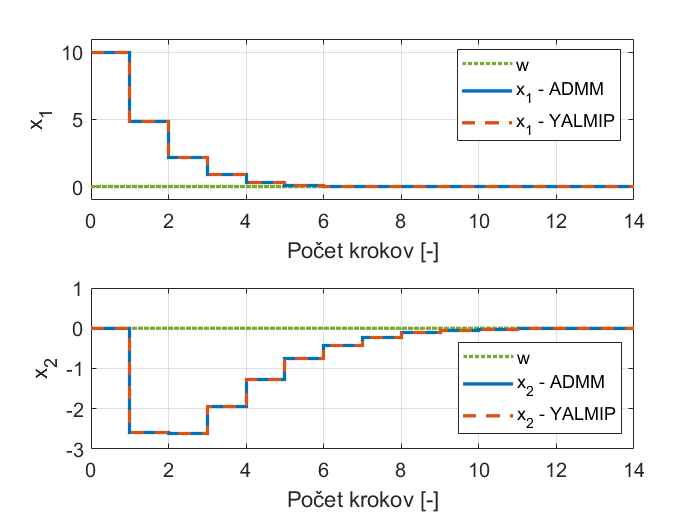
\includegraphics[width=13cm,height=10cm]{images/Hmotny_bod/Priebeh_riadenia}
	\caption{Priebeh riadenia pre lineárny systém}
	\label{fig1: PRLS}
\end{figure}
Ako môžeme vidieť na (Obr. 3.1), v oboch prípadoch sa nám podarilo dosiahnuť žiadanú veličinu (nulovú odchýlku stavov) a priebeh riadenia ja totožný pri oboch metódach.
\begin{figure}[H]
	\centering
	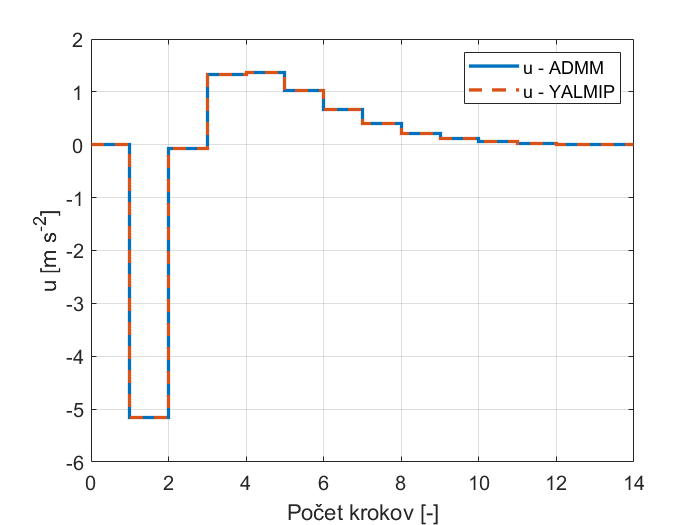
\includegraphics[width=13cm,height=10cm]{images/Hmotny_bod/Akcne_zasahy}
	\caption{Vývoj akčných zásahov}
	\label{fig2:AZLS}
\end{figure}
Rovnako ako stavy, tak aj akčné zásahy, sú totožné pri oboch metódach, čo môžeme vidieť na (Obr. 3.2).
\newpage
\begin{figure}[H]
	\centering
	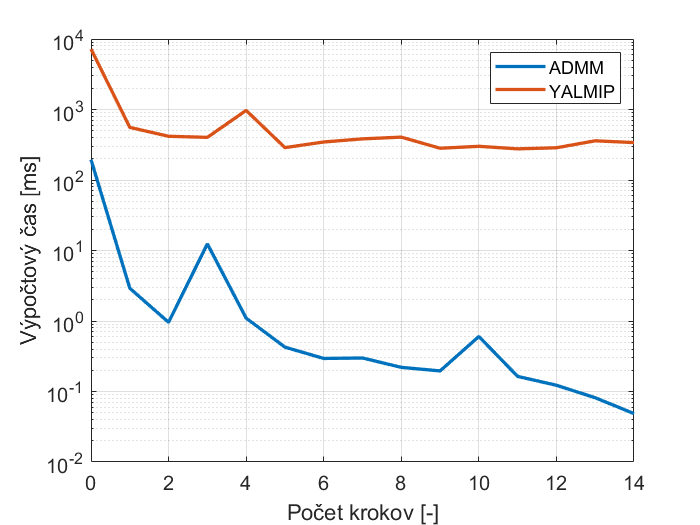
\includegraphics[width=13cm,height=10cm]{images/Hmotny_bod/Vypoctovy_cas}
	\caption{Porovnanie výpočtovej náročnosti MPC, medzi ADMM a YALMIP}
	\label{fig3: VNAA}
\end{figure}
Pre nás je najdôležitejší graf výpočtovej náročnosti (Obr. 3.3). Ako môžeme vidieť, podarilo sa nám dosiahnuť značné zlepšenie oproti analytickému riešiteľu z toolboxu YALMIP. Zatiaľ čo inicializačný čas pre ADMM bol okolo 100ms, najrýchlejšie riešenie pomocou YALMIP sa pohybovalo vyššie ako 100ms. Z tohoto porovnania vyplýva, že ADMM metóda je lepšia pre systémy s rýchlou dynamikou ($T_{s} \geq 1s $), ak sú opísané lineárnym matematickým modelom. 
\newpage


\section{Optimálne zastavenie DC motora}

DC motor je často využívaným zariadením v priemysle, ale aj v bežnom živote. Môže nadobúdať rôzne veľkosti a formy a jeho účelom je meniť elektrickú energiu na energiu mechanickú. Čo je pre nás dôležité, pracuje pod veľmi malou periódou vzorkovania. Je to teda systém s veľmi rýchlou dynamikou a nedá sa jednoducho riadiť pomocou nelineárneho MPC. 
\label{math:model_DC}
V tomto prípade budeme mať model systému opísaný nelineárnymi diferenciálnymi rovnicami, ktoré sú v nasledovnom tvare:
\begin{subequations}
	\begin{align}
	& \dot{x}^{(1)}(t) = - \frac{R}{L_{a}}x^{(1)}(t) - \frac{k_{m}}{L_{a}}u(t)x^{(2)}(t) + \frac{u_a}{L_a},\\
	& \dot{x}^{(2)}(t) = - \frac{B}{J}x^{(2)}(t) - \frac{k_{m}}{J}u(t)x^{(1)}(t) + \frac{\tau_l}{J},\\
	& y(t) = x^{(1)}(t),
	\end{align}
\end{subequations}
kde prvý stav $x^{(1)}$ predstavuje prúd rotora v $[A]$, druhý stav $x^{(2)}$ predstavuje uhlovú rýchlosť v $[rad/s]$ a vstupom $u$ je prúd statora udávaný v $[A]$. Naša sledovaná veličina bude uhlová rýchlosť (druhý stav)\cite{bib2}.
\begin{table}[h!]
	\centering
	\caption{Parametre DC motora \cite{bib2}}
	\label{tab.1: Parametre DC motora}
	\begin{tabular}{c c c}
		\hline
		\textbf{Značka} & \textbf{Hodnota} & \textbf{Veličina} \\ \hline
		$L_{a}$ & $0,314$ & $H$ \\ 
		$R_{a}$ & $12,345$ & $\Omega$ \\ 
		$k_{m}$ & $0,253$ & $N m A^{-2}$ \\ 
		$J$ & $0,00441$ & $N m s^{-2}$ \\ 
		$B_{a}$ & $ 0,00732$ & $N m s$ \\ 
		$\tau_l$ & $1,47$ & $N m$ \\
		$u_{a}$ & $60$ & $V$ \\ \hline
	\end{tabular}
\end{table}

Keďže máme model v kontinuálnej časovej oblasti, musíme si ho pretransformovať do diskrétnej podoby. Využijeme pri tom Eulerovu metódu, kde aproximujeme kontinuálny model diskrétnym podľa teórie, ktorú sme si uvideli v kapitole \hyperref[se:diskretizacia]{(2.2)}. Model systému po diskretizácií má nasledovnú podobu:
\begin{subequations}
\label{math:Dmodel_DC}
\begin{align}
& x_{k+1}^{(1)} = x^{(1)}_{k}+T_{s}\left(- \frac{R}{L_{a}}x^{(1)}_{k} - \frac{k_{m}}{L_{a}}u_{k}x^{(2)}_{k} + \frac{u_a}{L_a}\right),\\
& x_{k+1}^{(2)} = x^{(2)}_{k}+T_{s}\left(- \frac{B}{J}x^{(2)}_{k} - \frac{k_{m}}{J}u_{k}x^{(1)}_{k} + \frac{\tau_l}{J}\right),\\
& y(t) = x^{(1)}_{k},
\end{align}
\end{subequations}
kde $T_{s}$ je perióda vzorkovania , ktorú sme použili ako krok diskreditácie. Keďže sa jedná o veľmi rýchly systém, jeho perióda vzorkovania je veľmi malá, v našom prípade je to $T_{s} = 50ms$. Túto periódu musíme počas riadenia dodržiavať, ak chceme aby náš prediktívny regulátor bol stabilný a stihol vypočítať akčný zásah v každej perióde.

Našou úlohou je čo najefektívnejšie zastaviť DC motor z referenčných stavov, $x_{0}^{(1)}=0,887 A$ a $x_{0}^{(2)}=0,587 s^{-1}$, pričom nás fyzikálne obmedzuje vstup do systému $-4 \leq u_{k} \leq 4$. 

Ako prvé si zadefinujeme nelineárne MPC s ohraničeniami ($N = 5$), vo forme, ktorú sme si ukázali v kapitole  \hyperref[subse:NelinearneMPC]{(2.1.3)}. S nasledovnými váhovými maticami:
\begin{align}
	Q = \begin{bmatrix}
		1&0\\
		0&100
	\end{bmatrix}, 
	R = \begin{bmatrix}
	1
	\end{bmatrix}.
\end{align}
Pomocou logaritmickej bariéry si môžeme pridať ohraničenia do účelovej funkcie a vytvoríme si tak neohraničený optimalizačný problém. Pre podrobnejšie vysvetlenie si môžeme pozrieť kapitolu \hyperref[subse:Ohranicenia]{(2.5.3)}. Ďalej riešime problém bez ohraničení, ako sme popísali v časti \hyperref[subse:Nelin_MPC_ADMM]{(2.5.2)}. Rozdistribuujeme si MPC na $N$ predikčných horizontov, pridáme duálne funkcie a vytvoríme si rozšírený lagrangean. Rovnako ako v predošlej simulácii, kritériá pre zastavenie \hyperref[subse:ADMM2]{iterácií v ADMM} sme zvolili presnosť hľadaných počiatočných stavov $\norm{x_{k}(x_{k-1},u_{k-1})- x_{k}} < \epsilon,\hspace{0.5cm} k=1,\dots,N-1$ a taktiež veľkosť zmeny predikovaných akčných zásahov $\norm{u_{k}^{(i-1)}-u_{k}^{(i)}} < \epsilon,\hspace{0.5cm} k=0,\dots,N-1$, kde $\epsilon = 1\mathrm{e}{-5}$. Pre porovnanie výsledkov normálneho MPC a decentralizovaného MPC sme vytvorili simuláciu na diskrétnom nelineárnom modeli, \hyperref[math:Dmodel_DC]{rovnice (3.6)}.
\begin{figure}[H]
	\centering
	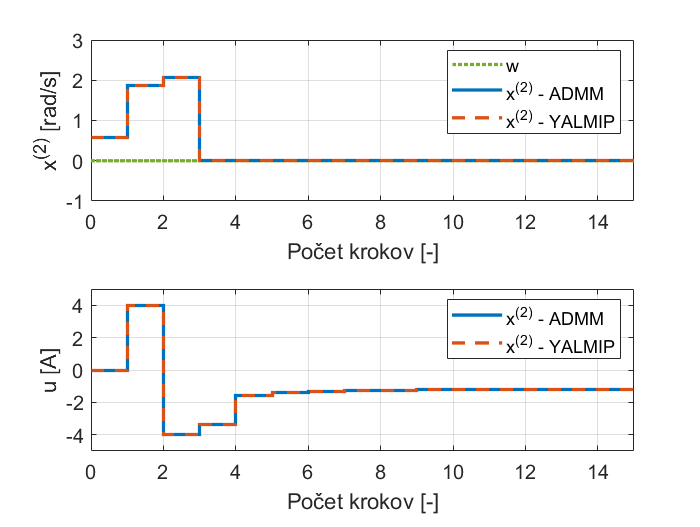
\includegraphics[width=13cm,height=10cm]{images/DC_motor/Priebeh_riadenia_a_akcne_zasahy}
	\caption{Priebeh riadenia DC motora}
	\label{fig7: PR}
\end{figure}
Ako môžeme vidieť na (Obr 3.4), v oboch prípadoch sa nám podarilo dosiahnuť žiadanú veličinu (zastavenie DC motora) s totožným priebehom riadenia. Vývoj stavu $x^{(1)}$ čo je prúd rotora nás nezaujíma a preto ho nemáme ani zobrazený.
\newpage
\begin{figure}[H]	
	\centering
	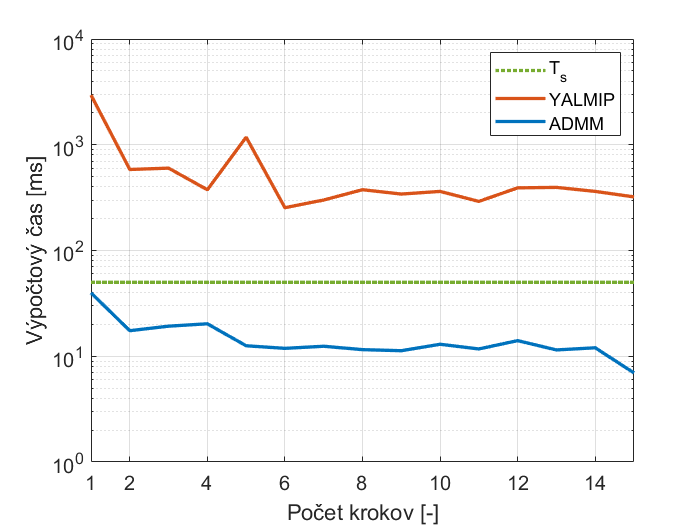
\includegraphics[width=13cm,height=10cm]{images/DC_motor/Vypoctovy_cas}
	\caption{Porovnanie výpočtovej náročnosti MPC, medzi ADMM a YALMIP}
	\label{fig9: VN}
\end{figure}
Na (Obr. 3.5) si môžeme všimnúť, že pomocou analytického riešiteľa z toolboxu YALMIP sme sa ani len nepriblížili k perióde vzorkovania DC motora, a preto nie je možné používať takýto spôsob výpočtu MPC pre riadenie daného systému. Naopak, pomocou ADMM sa nám podarilo dosiahnuť veľmi dobré výsledky. Vďaka ADMM sme mohli rozdeliť jeden optimalizačný problém na päť decentralizovaných a riešiť ich samostatne. Takéto rozdelenie zmenšilo počet iterácií v Newtonovej numerickej optimalizácii a zároveň umožnilo paralelné riešenie týchto decentralizovaných problémov. Vo výsledku vidíme, že sa nám podarilo dostatočne zrýchliť výpočet akčných zásahov a stíhame ich opakovane počítať v rámci periódy vzorkovania $T_{s} = 50ms$.

\chapter{Aplikácia}
\label{part:Aplikacia}

V tejto poslednej kapitole sa budeme venovať návrhu aplikácie, pomocou ktorej môžeme využívať decentralizované MPC s možnosťou paralelného riešenia na viacerých výpočtových zariadeniach. V rámci aplikácie bude možné pracovať s rôznymi lineárnymi aj nelineárnymi modelmi systému. Výstupom z aplikácie bude vypočítaný optimálny akčný zásah v danej perióde vzorkovania. Ďalej budeme využívať tento výstup pri simulácií riadenia na definovanom modeli systému. Alternatívou by bolo nahradenie simulácie reálnym systémom, ale bolo by nutné zaviesť úpravy. 

Najskôr si ukážeme architektúru aplikácie, na základe ktorej sme neskôr vybudovali logiku celej aplikácie. V ďalšej časti si vysvetlíme nastavenie servera, ako s ním budeme komunikovať a spôsob ukladania dát v aplikácii. Následne na to si ukážeme rozhranie, s ktorým sa stretne používateľ. A posledné dve časti tejto kapitoly budú venované spôsobu fungovania aplikácie, rozoberieme si postupnosť logických krokov a overíme si ich na simulácií. 
\section{Architektúra aplikácie}
Aplikáciu delíme na dve časti, prvá je serverová a bude naprogramovaná v jazyku Python pomocou knižnice Flusk. Druhú časť nazývame klientská a bude sa nachádzať vo webovom rozhraní.
\label{fig:ArchitekturaAPK}
\begin{figure}[H]	
	\centering
	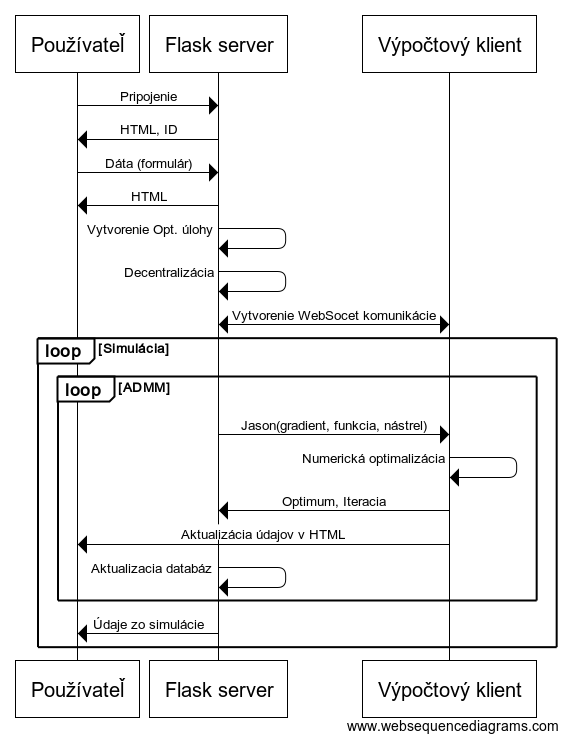
\includegraphics[width=13cm,height=18cm]{images/Aplikacia}
	\caption{Zjednodušený diagram aplikácie pre jedného klienta}
\end{figure}
\newpage
Na (Obr. 4.1) môžeme vidieť architektúru, ktorá slúžila ako základ pre našu aplikáciu. Klientská čast sa bude deliť na dve, prvá je používateľské rozhranie v ňom bude klient môcť ovládať simuláciu a sledovať výsledky z optimalizácie. Druhá časť je takzvaný výpočtový klient, táto časť bude reprezentovať numerickú optimalizáciu, ktorá bude prebiehať na pozadí prehliadača v JavaScripte. 
\section{Server}
Ako sme už spomínali, pre vytvorenie servera použijeme knižnicu Flask. Táto knižnica obsahuje micro web framwork pre programovací jazyk Python, inak povedané, podporuje vývoj webovej aplikácie, konkrétne web server. Nazývaný je micro, lebo je navrhnutý tak, aby jeho jadro bolo čo najjednoduchšie, ale podporuje rozšíriteľnosť pomocou už existujúcich knižníc. To je zároveň aj jeho najväčšia výhoda, nie je dopredu určené, aký druh databáz musíme používať, alebo v akej forme budeme odosielať a prijímať dáta, vo všetkom má developer voľnosť.
\subsection{Nastavenie servera}
Nastavenie servera je veľmi jednoduché, stačí importovať knižnicu Flask,
\begin{lstlisting}[language=Python]
from flask import Flask
\end{lstlisting}\noindent
vytvoríme si premennú, ktorá bude reprezentovať náš server.
\begin{lstlisting}[language=Python]
app = Flask(__name__)
\end{lstlisting}\noindent
Ďalej je potrebné určiť, čo sa stane, keď sa klient pripojí na server. V nasledujúcom príklade odkážeme klienta na html stránku
\begin{lstlisting}[language=Python]
@app.route('/')
	return render_template('index.html')
\end{lstlisting}\noindent
a nakoniec si zadefinujeme, na akom porte bude náš server fungovať.
\begin{lstlisting}[language=Python]
if __name__ == '__main__':
	app.run(host='localhost', port=5000)
\end{lstlisting}
Takto nastavený server nájdeme na adrese http://localhost:5000/ rovnako ako náš, ktorý budeme poožívať v tomto projekte.

\subsection{Práca s databázou}
Vďaka voľnosti, ktorú nám poskytuje Flask, sme si mohli vybrať zo širokej škály knižníc pre prácu s dátami. V dnešnej dobe sú databázy najpoužívanejšou a veľmi efektívnou formou, ako ukladať, aktualizovať a spravovať údaje. Takto uložené dáta sú v tabuľkovej podobe, kde každý stĺpec má preddefinovaný formát a veľkosť a každý riadok stĺpca má priradený jedinečný index, ktorý uľahčuje SQL (Structured Query Language) prehľadávanie v databáze.

My sme v tejto práci využili knižnicu SQLAlchemy, konkrétne jej upravenú verziu FlaskSQLAlchemy. Umožňuje plné využívanie SQL pre prácu s databázami v našom Flask serveri, a to pomocou takzvaného ORM (Object Relational Mapper), čo je programovacia technika pre konvertovanie dát medzi nekompatibilnými systémami (programovacími jazykmi), čo je v našom prípade Python a SQL. 

Pomocou tejto knižnice sme si vytvorili štyri databázy, ktoré budeme používať v našej aplikácii. 
\label{DB:Klient}
\begin{enumerate}
\item{ Databáza klientov - v tejto databáze budeme mať uložených všetkých klientov, ktorý pracujú alebo pracovali na optimalizácii, štruktúra databázy je nasledovná.
\begin{lstlisting}[language=Python]
class Clients(db.Model):
__bind_key__ = 'Clients'
ID = db.Column(db.Integer, primary_key=True)
MPC_optimization_id = db.Column(db.Integer, index=True)
Date_created = db.Column(db.DateTime,\
                      default=datetime.utcnow)
Status = db.Column(db.Integer(2), index=True) 
\end{lstlisting}
}
\label{DB:OPT}
\item{ Databáza optimalizačných úloh - táto databáza bude obsahovať všetky optimalizačné problémy (MPC), ktoré si vytvoríme zo zadefinovaných informácií od klienta. Budeme ju ďalej používať ako základ pre decentralizovanú optimalizáciu. Hlavnou vlastnosťou tejto databázy bude, že sa naplní iba raz v rámci jedného MPC a tieto údaje budú nemenné počas chodu aplikácie. Obsahuje nasledovné informácie.
\begin{lstlisting}[language=Python]
class MPC_optimization(db.Model):
__bind_key__ = 'MPC_optimization'
ID = db.Column(db.Integer, primary_key=True)
General_Model = db.Column(db.String(5000), index=True)
General_Function = db.Column(db.String(10000), index=True)
Variable = db.Column(db.String(64), index=True)
Reference = db.Column(db.String(64), index=True)
Nmin = db.Column(db.String(64), index=True)
Nmax = db.Column(db.String(64), index=True)
Client_id = db.Column(db.Integer, index=True)
Status = db.Column(db.Integer(2), index=True)
\end{lstlisting}
}
\label{DB:WORKER}
\item{ Databáza distribuovaných optimalizačných úloh - táto databáza bude niesť informácie o distribuovanej optimalizačnej úlohe pre jednotlivých klientov. Na rozdiel od predošlej databázy, táto sa môže meniť počas chodu aplikácie, ale len vtedy, ak sa pripojí alebo odpojí klient z aplikácie. Databáza bude mať zadefinovanú nasledovnú podobu. 
\begin{lstlisting}[language=Python]
class MPC_Worker(db.Model):
__bind_key__= 'MPC_Worker'
ID = db.Column(db.Integer, primary_key=True)
Optimization_Variables = db.Column(db.String(64), index=True)
Function = db.Column(db.String(5000), index=True)
Gradient = db.Column(db.String(10000), index=True)
Client_id = db.Column(db.Integer, index=True)
Status = db.Column(db.Integer(2), index=True)
\end{lstlisting}
}
\label{DB:WORKER_DATA}
\item{ Databáza výsledkov po optimalizácii - posledná databáza, s ktorou budeme pracovať v rámci tejto aplikácie. Na rozdiel od predošlých databáz, táto sa vytvorí pre každú optimalizovanú premennú a bude sa aktualizovať po každej optimalizácii. Štruktúra databázy je nasledovná.
\begin{lstlisting}[language=Python]
class MPC_Worker_data(db.Model):
__bind_key__= 'MPC_Worker_data'
ID = db.Column(db.Integer, primary_key=True)
Variable = db.Column(db.String(64), index=True)
Optimal_value = db.Column(db.String(20), index=True)
Iteration = db.Column(db.Integer(20), index=True)
Client_id = db.Column(db.Integer, index=True)
Status = db.Column(db.Integer(2), index=True)
\end{lstlisting}
}
\end{enumerate}

\subsection{Komunikácia}
Komunikácia medzi serverom a klientom bude prebiehať dvoma rôznymi spôsobmi. Pre jednorázové akcie, ako je odoslanie formulára alebo pripojenie či odpojenie zo servera, využijeme HTTP requesty, konkrétne metódy POST a GET. Pre častú komunikáciu ako bude odosielanie dát na optimalizáciu alebo zmena referencie v simulácii je omnoho lepšou možnosťou otvoriť komunikačný kanál medzi serverom a klientom. Tento kanál bude sprostredkovávaný pomocou WebSocket protokolu a zjednoduší komunikáciu. Server tak bude môcť rovno odosielať dáta klientovi, bez toho aby o ne musel najskôr požiadať. 

\subsubsection{HTTP}
HTTP je skratka z angličtiny (Hypertext Transfer Protocol) a predstavuje protokol, ktorý bol určený na výmenu hypertextových dokumentov medzi serverom a prehliadačom (klientom). Funguje na nasledovnom princípe, klient zašle požiadavku (request) a čaká na odpoveď zo strany servera, ktorý odpovedá zaslaním HTML súboru alebo iného obsahu, môže vykonať nejakú funkciu či odpovedať správou späť klientovi. 

HTTP poskytuje viacero request metód, ktoré hovoria o tom, akú odpoveď očakáva klient zo strany servera. My budeme využívať dve najpoužívanejšie metódy.
\begin{enumerate}
\item { Metóda GET, zjednodušene povedané, slúži na vyžiadanie si dát zo špecifického zdroja. Táto požiadavka ostáva v histórii prehliadača a nemala by sa využívať pri práci s citlivými údajmi. V našej aplikácií ju budeme využívať pre presmerovanie klienta medzi HTML súbormi.  
}
\item { Metóda POST, sa využíva najmä pre odoslanie, vytváranie alebo aktualizovanie dát pre server. Táto požiadavka neostáva v histórii. My ju budeme využívať pre potvrdenie a odoslanie formulárov z webovej stránky na server.  
}
\end{enumerate}

\subsubsection{WebSockets}
WebSockets je iná forma prijímania a odosielanie dát medzi serverom a prehliadačom ako tomu bolo pri HTTP. Poskytuje komunikáciu v oboch smeroch (klient-server) cez jediné TCP (Transmission Control Protocol) pripojenie. Pomocou WebSocekt aplikácie vieme vytvoriť obojstrannú komunikáciu, kde klient môže cez prehliadač poslať správy (dáta) na server a tiež môže dostať odpoveď od servera na základe nejakých udalostí bez toho, aby o ne musel požiadať.

Na rozdiel od HTTP, na vytvorenie takejto komunikácie budeme potrebovať dve knižnice, jednu pre Flask server a druhú pre klienta (JavaScript). Na strane servera budeme využívať flask-SocetIO, táto knižnica nám zmení nastavenia servera (konkrétne definovanie portu) a to tak, že nám obalí pôvodný server. Zmena bude nasledovná.
\begin{lstlisting}[language=Python]
from flask_socketio import SocketIO
socketio = SocketIO(app)
if __name__ == '__main__':
	socketio.run(app, host='localhost', port=5000)
\end{lstlisting}
Pre JavaScript použijeme knižnicu Socet.IO, ktorú si pridáme pomocou webového linku. Je nutné sa pripojiť na adresu, kde bude komunikácia prebiehať, v našom prípade je to adresa servera.
\begin{lstlisting}[language=Java]
var socket = io.connect('http://localhost:5000/');
\end{lstlisting}

\section{Klientská časť}
Na strane klienta budeme mať jednoduché rozhranie, kde bude klient navádzaný pomocou tlačidiel a formulára na zadefinovanie MPC. Akonáhle sa odošlú údaje na server, klient bude presmerovaný na HTML stránku, kde už bude mať k dispozícií všetky informácie o optimalizácii a simulácii. Aby bola klientska časť zovšeobecnená, budeme vo webovom rozhraní používať iba anglický jazyk. V nasledujúcich dvoch častiach bude ukázané, s akým rozhraním sa klient stretne a okrajovo bude naznačené, čo sa bude vykonávať v JavaScripte, teda na pozadí stránky. V nasledujúcej podkapitole (4.3) si tieto veci viac priblížime. 
\subsection{Formulár}
\label{subse:Formular}
V tejto aplikácii budeme využívať iba jeden formulár. Ten sme si rozdelili na dve časti. V prvej sa zadefinuje model riadeného systému a všetky vstupné, výstupné a stavové premenné. Druhá čast slúži na definovanie optimalizačného problému (parametre prediktívneho regulátora). Všetky polia sa vypĺňajú pomocou maticového zápisu, rovnako ako v programovacom jazyku Matlab. Formulár sa po vyplnení odošle pomocou HTTP metódy POST na server, kde sa spracujú všetky informácie. 
\begin{enumerate}
\item {Nastavenie riadeného systému- v tomto formulári môžeme zadefinovať diskrétny model systému, buď ako stavový opis (lineárny model) alebo pomocou diferenciálnych rovníc (lineárny/nelineárny model).
\begin{figure}[H]	
	\centering
	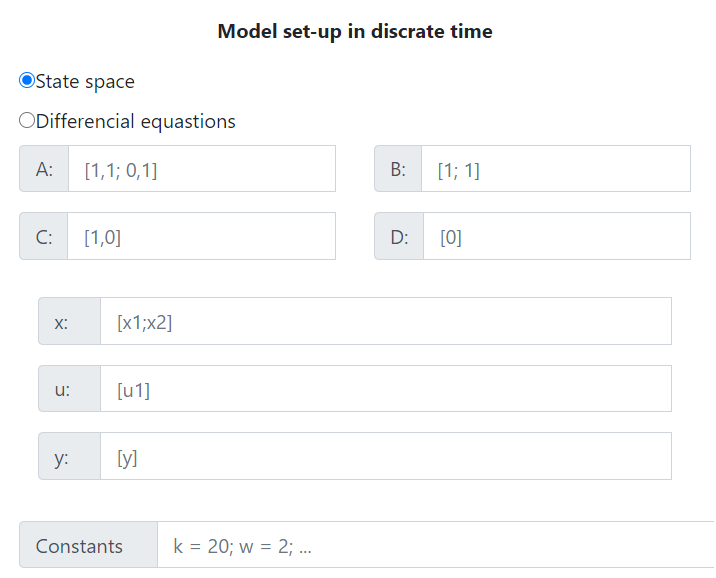
\includegraphics[width=11cm,height=8cm]{images/Model_setup}
	\caption{Formulár pre definovanie systému}
\end{figure}
V ľavom hornom rohu (Obr. 4.1) si môžeme vybrať z týchto dvoch možností a na základe výberu sa nám upravia vstupné polia. Na obrázku vyššie máme znázornený stavový opis systému, kde si zadefinujeme matice A a B. Ako sme už spomínali, v tomto projekte budeme uvažovať iba stavové riadenie, takže rovnica výstupu $y_{k} = Cx_{k} + Du_{k}$ nás nebude zaujímať, polia sú vytvorené pre prípadné zmeny v budúcnosti. V poliach x a u, zadefinujeme vstupné (u) a stavové (x) veličiny, môžu to byť ľubovolné názvy, ale pri použití diferenciálnych rovníc sa musia zhodovať s tým v rovniciach. Posledné pole pre konštanty slúži na definovanie konštánt, ktoré sa použili v poliach vyššie. Teda je možné predísť písaniu čísel do rovníc a môžeme ich nahradiť premennými. 
}
\item {Definovanie parametrov MPC.
\begin{figure}[H]	
	\centering
	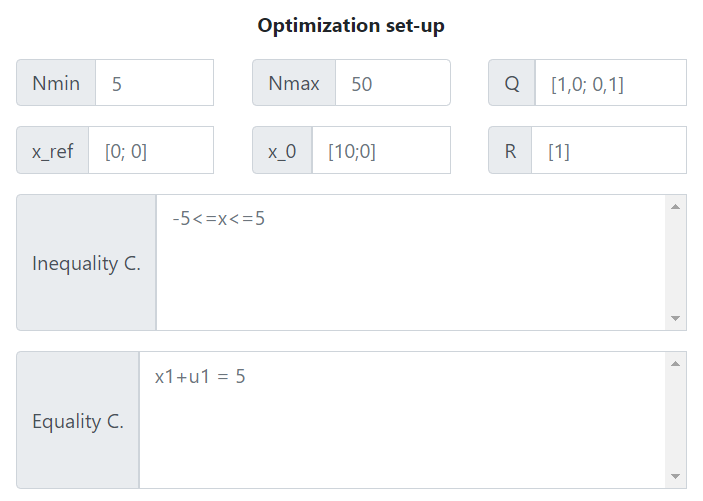
\includegraphics[width=11cm,height=8cm]{images/MPC_setup}
	\caption{Formulár pre definovanie MPC}
\end{figure}
Ako môžeme vidieť na (Obr. 4.2) máme celkovo osem polí pre definovanie predikatívneho regulátora, z toho dve nebudeme v tomto projekte používať a to $Nmax$, čo predstavuje maximálny predikčný horizont a rovnostné ohraničenia (Equality C.). Prvé pole $Nmin$ definuje minimálny predikčný horizont, $Q$ a $R$ sú váhové matice používané v MPC. Ďalej máme pole určené pre neostré nerovnostné ohraničenia (Inequality C.) a dve polia pre definovanie počiatočnej hodnoty stavov ($x_{0}$) a referencie, kam sa majú jednotlivé stavy dostať ($x_{ref}$).
}
\end{enumerate}
Súčasťou tohoto formulára je tiež validácia, ktorá sa spustí vždy pri odosielaní formulára. Prebieha v JavaScripte na strane klienta. Kontroluje, či sú zadefinované všetky potrebné polia a zároveň kontroluje, či majú všetky správne rozmery. Ak formulár neprejde validáciou, nebude odoslaný ďalej na server, a vyskočí okno pri danom poli s popisom chyby.
\subsection{Optimalizácia a simulácia}
\label{subse:OPTaSIM}
Akonáhle sa odošlú údaje z formulára časť \hyperref[subse:Formular]{(4.3.1)} na server, klient je presmerovaný na novú HTML stránku. Na tejto stránke bude v pozadí prebiehať Newtonova numerická optimalizácia  \hyperref[opt:Newton]{(2.5.2)}, táto optimalizácia bude naprogramovaná v jazyku JavaScript. Jej úlohou bude nájsť optimálne riešenie pre decentralizovaný optimalizačný problém. Výsledky z tejto optimalizácie budú zobrazené na stránke v nasledujúcom formáte. 
\label{fig:Tabulka}
\begin{figure}[H]	
	\centering
	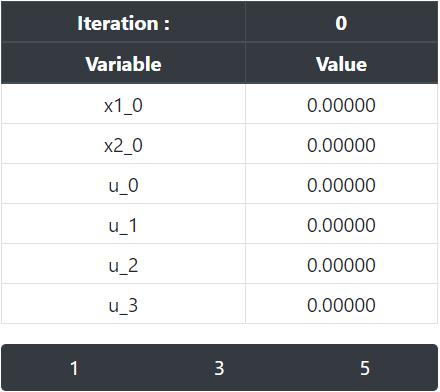
\includegraphics[width=6cm,height=6.5cm]{images/tabulka}
	\caption{Tabuľka výsledkov}
\end{figure}
Na (Obr. 4.3) môžeme vidieť príklad dynamickej tabuľky. Táto tabuľka zobrazuje všetky optimalizované premenné a ich hodnoty z jednotlivých optimalizácií. V tabuľke tiež môžeme nájsť, koľko iterácií trvalo numerickej optimalizácii, kým skonvergovala do optima. Po ukončení simulácie si môžeme pozrieť jednotlivé výsledky zo všetkých optimalizácií, ktoré klient vykonal a to pomocou tlačidiel nachádzajúcich sa pod tabuľkou.

Súčasťou tejto stránky je tiež zobrazenie simulácie riadeného systému. Táto simulácia prebieha na serveri, bude možné ju ovládať, a to pomocou zmeny referencie a zastavovacieho tlačidla.
\begin{figure}[H]	
	\centering
	
\includegraphics[width=9cm,height=1cm]{images/ovladanie_simulacie}
	\caption{Panel pre ovládanie simulácie}
\end{figure}
Na (Obr. 4.4) máme zobrazený panel, pomocou ktorého môžeme ovládať simuláciu zo strany klienta. Máme k dispozícii možnosť zastaviť prebiehajúcu simuláciu, alebo zmeniť žiadanú hodnotu pre jednotlivé stavy. Rovnako, ako v predchádzajúcej časti, aj tu sa zvalidujú údaje pred odoslaním. Ak prejdú validáciou, sú odoslané na server, kde sú spracované. Server odošle naspäť správu, či všetko prebehlo v poriadku.

Pre sledovanie simulácie budeme mať k dispozícii dva dynamické grafy, ktoré budú zobrazovať údaje v reálnom čase, a to pomocou JavaScript knižnice Chart.js. Táto knižnica je voľne dostupná na internete, bude nám poskytovať možnosť vytvorenia interaktívnych grafov a veľkú voľnosť, vďaka ktorej môžeme premeniť statické grafy na dynamické. Nad grafom bude zobrazená legenda s príslušnými veličinami, a tiež bude fungovať ako panel ovládania, pomocou ktorého môžeme pridávať a odoberať veličiny z grafu. 
\begin{figure}[H]
	\centering
	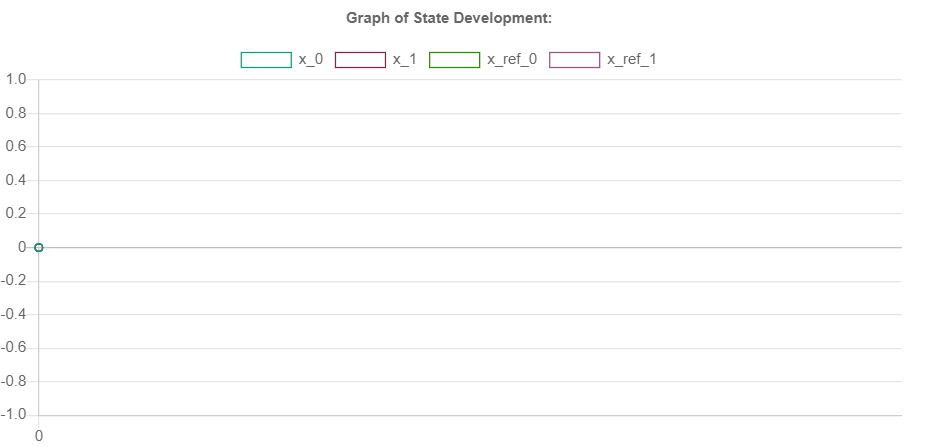
\includegraphics[width=13cm,height=6cm]{images/graf_stavov}
	\caption{Vývoj stavov počas riadenia}
\end{figure}
Na grafe vyššie (Obr. 4.5) bude zobrazený priebeh riadenia jednotlivých stavov a ich referencie.
\begin{figure}[H]	
	\centering
	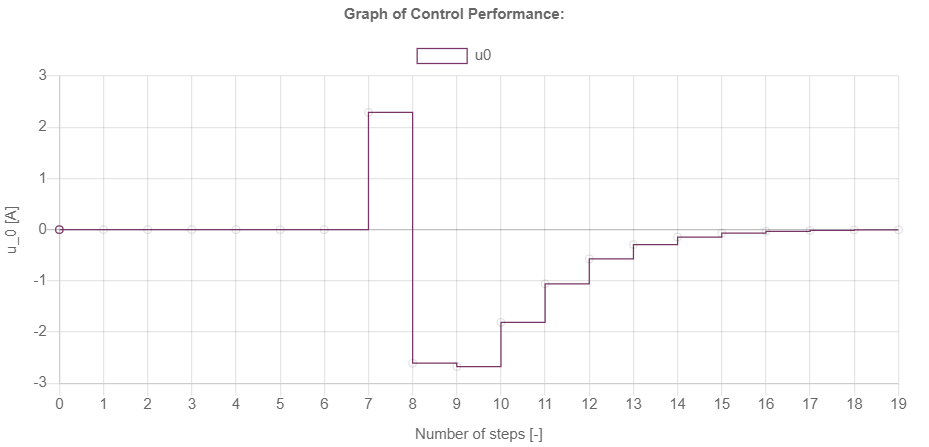
\includegraphics[width=13cm,height=6cm]{images/graf_vstupov}
	\caption{Vývoj akčných zásahov počas riadenia}
\end{figure}
Druhý graf, ktorý budeme mať k dispozícii, je graf vstupov do systému. Bude nám slúžiť pre sledovanie akčných zásahov z MPC.

\section{Logická postupnosť aplikácie}
V tejto podkapitole si rozoberieme rozloženie aplikácie a podrobne si vysvetlíme jej logickú postupnosť. Na \hyperref[fig:ArchitekturaAPK]{(Obr. 4.7)} sme si mohli pozrieť zjednodušený diagram našej aplikácie. Zjednodušený preto, lebo obsahuje iba najhlavnejšie akcie, ktoré sa vykonávajú v aplikácii a je zobrazený iba jeden klient, ktorý otvoril MPC. My si však ideme vysvetliť podrobnejšiu schému, kde si detailne rozoberieme aj menšie akcie a budú v nej zapojení viacerí klienti.
\begin{description}
\item[1. Klient 1:]{\hfill
	\begin{enumerate}
		\item{
			Klient sa pripojí na http://localhost:5000/, pomocou tlačidla si vyberie prediktívne riadenie (Model Predictive Control), odošle GET request na server. Sever vytvorí nový záznam v \hyperref[DB:Klient]{databáze klientov} a priradí mu vlastné ID. Ako odpoveď mu vráti HTML stránku, kde bude mať na výber vytvoriť nové prediktívne riadenie (New Model Predictive Control), po stlačení bude rovnako presmerovaný na formulár.
		}
		\item{
			Ako sme popísali v časti \hyperref[subse:Formular]{(4.3.1)}, klient bude musieť zadefinovať všetky potrebné parametre MPC a všetky potrebné polia pre definovanie modelu systému. Potvrdením sa formulár zvaliduje, ak prejde validáciou je odoslaný na server pomocou request metódy POST.
		}
	\end{enumerate}
}
\item[2. Server:]{\hfill
	\begin{enumerate}
		\item{
			Server spracuje prijaté dáta z formulára, na základe toho či príde diferenciálna rovnica alebo stavový opis systému, upraví tieto rovnice a vytvorí všeobecný model systému. Ostatné dáta sú spracované z textovej podoby do použiteľnej formy.
		}
		\item{
			Následne sú dáta využité pre vytvorenie účelovej funkcie podľa všeobecného vzoru, ktorý sme si ukázali v časti \hyperref[subse:MPC]{(2.1.1)} pre definovaný predikčný horizont $Nmin$. Ak sú zadefinované ohraničenia, tak sa pridajú do účelovej funkcie podľa teórie, ktorú sme si ukázali v časti \hyperref[subse:Ohranicenia]{(2.5.3)}. V ďalšom kroku sa vytvorí nový záznam v \hyperref[DB:OPT]{databáze optimalizačných úloh} so všeobecnými informáciami od Klienta 1.
		}
		\item{
			 Ako posledná úprava sa do účelovej funkcie dosadí vytvorený všeobecný model systému v konkrétnych predikčných horizontoch. Potom sa vytvorí gradient účelovej funkcie vzhľadom k optimalizovaným premenným a vygenerujú sa počiatočné nástrely. Z takýchto údajov sa vytvorí prvý záznam v \hyperref[DB:WORKER]{databáze distribuovaných optimalizačných úloh} a tiež záznam pre každú premennú v \hyperref[DB:WORKER_DATA]{databáze výsledkov po optimalizácií}. Vzhľadom na to, že je prihlásený iba jeden klient, bude sa jednať o normálne centralizované MPC.
		}
		\item{
			Ako odpoveď na prijaté dáta z formulára server vráti HTML stránku spolu s informáciou o IDčku klienta.
		}
	\end{enumerate}
}
\item[3. Klient 1:]{\hfill
\begin{enumerate}
\item{
Klient je na poslednej, a zároveň hlavnej HTML stránke, ktorú sme si predstavili v časti \hyperref[subse:OPTaSIM]{(4.3.2)}. Ako prvé sa pripojí cez JavaScript na WebSoket kanál, kde bude odosielať a dostávať správy.
}
\item{
Cez tento komunikačný kanál zašle serveru správu, že je pripravený na prijatie dát. Server mu odpovie zaslaním dát z databáz v podobe Jason
\begin{lstlisting}[language=Python]
{"Klient_ID":[Gradient, Premenna, Hodnota, Funkcia]}
\end{lstlisting}
}
\item{Po obdržaní dát, sa zavolá funkcia pre numerickú optimalizáciu a tá vyrieši optimalizačný problém. Výsledok po optimalizácii sa pošle cez WebSocet kanál na sever a následne sa tento výsledok objaví v \hyperref[fig:Tabulka]{tabuľke výsledkov}.}
\end{enumerate}
}
\item[4. Server:]{\hfill
\begin{enumerate}
\item{
Server dostane dáta a aktualizuje \hyperref[DB:WORKER_DATA]{databázu výsledkov po optimalizácií}. Keďže je stále pripojený iba jeden klient, nemáme distribuovanú optimalizačnú úlohu, teda nevyužívame ani ADMM. V takejto situácii považujeme obdržané dáta za optimálne akčné zásahy z MPC.
}
\item{
Server zavolá simuláciu, pomocou vypočítaných akčných zásahov a počiatočných stavov vypočíta nové stavy a aktualizuje ich v \hyperref[DB:WORKER_DATA]{databáze výsledkov po optimalizácií}.
}
\item{
Ako posledný krok vytvorí nové dáta pre optimalizáciu z databázy v podobe Jason a odošle ich cez komunikačný kanál klientovi.
}
\end{enumerate}
}
\item[5. Klient 1:]{\hfill
	\begin{enumerate}
		\item{Klient opäť obdrží dáta, zavolá sa funkcia pre numerickú optimalizáciu, tá vyrieši optimalizačný problém. Výsledok po optimalizácii sa pošle cez WebSocet kanál na sever a následne sa tento výsledok objaví v \hyperref[fig:Tabulka]{tabuľke výsledkov}.}
	\end{enumerate}
}
\item[6. Cyklus:]{\hfill
	\begin{enumerate}
		\item{V tomto momente vznikne cyklus (od kroku 4. po 5.) a bude sa opakovať, až kým sa nepripojí nový klient.}
	\end{enumerate}
}
\item[7. Klient 2:]{\hfill
	\begin{enumerate}
		\item{Rovnako ako klient 1 sa aj klient 2 pripojí k serveru na adrese http://localhost:5000/,  pomocou tlačidla si vyberie prediktívne riadenie. V tomto okamžiku má na výber už z dvoch možností, pripojiť sa k prebiehajúcemu riadeniu (talčidlo Join MPC), alebo môže založiť ďalšie riadenie rovnako ako klient 1. Ak by si vybral zloženie nového riadenia, pokračoval by rovnako ako klient 1.}
		\item{
			Po pripojení sa k prebiehajúcemu riadeniu, odošle serveru request a ten mu pošle naspäť HTML stránku a priradí mu ID.
		}
		\item{ 
			Pripojí sa na komunikačný kanál a zašle serveru informáciu o tom, že sa pridal k riadeniu. 
		}
	\end{enumerate}
}
\item[8. Server :]{\hfill
	\begin{enumerate}
		\item{
			Server obdrží správu, že sa pripojil ďalší klient k riadeniu a preruší cyklus v korku 6.
		}
		\item{
			Zavolá \hyperref[DB:OPT]{databázu optimalizačných úloh} a nájde príslušné MPC, ku ktorému sa klient pripojil. Následne na to si zistí, koľko klientov je aktívnych a aký je $Nmin$ (minimálny predikčný horizont). Na základe tejto informácie vytvorí decentralizovaný optimalizačný problém zo všeobecnej rovnice a modelu systému. Postupuje podla teórie uvedenej v časti \hyperref[subse:Nelin_MPC_ADMM]{(2.5.2)} s výnimkou, že sa nebude uvažovať plná decentralizácia, ale rozdelí sa príslušný počet predikčných horizontov medzi klientov.
		}
		\item{
			Po vytvorení distribuovaného optimalizačného problému sa aktualizuje \hyperref[DB:WORKER]{databáza distribuovaných optimalizačných úloh} a \hyperref[DB:WORKER_DATA]{databáza výsledkov po optimalizácii}. S drobnou obmenou sa ako nástrel pre optimalizáciu využijú staré údaje a nebudú sa generovať nové. 
		}
		\item{
			Po aktualizácii údajov server zašle dáta cez komunikačný kanál všetkým klientom vo formáte Jason.
		}
	\end{enumerate}
}
\item[9. Cyklus:]{\hfill
	\begin{enumerate}
		\item{V tomto momente vznikne nový cyklus, ale komplikovanejší ako bol v kroku 6., pridá sa totiž ADMM k simulácii (budeme mať cyklus v cykle)}
		\item{Klienti obdržia dáta, zavolajú funkciu pre numerickú optimalizáciu a tá vyrieši optimalizačný problém. Výsledok po optimalizácii sa pošle cez WebSocet kanál na sever a následne sa tento výsledok objaví v \hyperref[fig:Tabulka]{tabuľke výsledkov}.}
		\item{
			Server čaká, kým neobdrží výsledky od všetkých klientov. Potom spracuje výsledky, aktualizuje databázy a duálnu funkciu. Následne na to vyhodnotí kritériá pre zastavenie ADMM. Ak nie sú splnené, pošle aktualizované dáta klientom a pokračuje od korku 2 (9. Cyklu). Ak sú kritériá splnené, považujeme výsledok za optimálne akčné zásahy. Ďalej server zavolá simuláciu pomocou vypočítaných akčných zásahov a počiatočných stavov, vypočíta nové stavy a aktualizuje ich v \hyperref[DB:WORKER_DATA]{databáze výsledkov po optimalizácii} a pokračuje od kroku 2 (9. Cyklu).
		}
	\end{enumerate}
}
\end{description}
Vysvetlili sme si princíp fungovania aplikácie pri pripojení dvoch klientov. Ak by sa pripojilo viac, než dvaja klienti, nespôsobí to problém, a postup bude vždy rovnaký od korku 7. Zmena môže nastať v dvoch prípadoch.
\begin{enumerate}
	\item{
	 Pripojí sa viac klientov ako je minimálny predikčný horizont, v takom prípade už máme maximálne decentralizovaný optimalizačný problém. Zmena nastane v tom, že sa nemá už aký predikčný horizont prideliť klientovi, a teda sa vytvorí nový predikčný horizont nad rámec minimálneho predikčného horizontu.
	}
	\item{
	Ak sa nejaký klient odpojí z riadenia, preruší sa cyklus v korku 9., na čo server zareaguje ako pri pridaní klienta do riadenia (krok 8.), len miesto toho, aby prepočítal distribúciu optimalizácie o klienta navyše, odoberie jedného. 
	}
\end{enumerate}
Celú aplikáciu sme zverejnili githube spolu s možnosťou vytvorenia docker súboru.  Ten umožňuje spustenie servera na hocikom operačnom systéme a nie je nutné mať nainštalované, žiadne programovacie jazyky alebo špeciálne knižnice.

\section{Experiment}
V poslednej časti tejto kapitoly overíme funkčnosť navrhnutej aplikácie na simulácii, a to pri rovnakých podmienkach, ako v časti \hyperref[sec:HB]{(3.1)}. Prihlásime prvého klienta, ten zadefinuje všetky potrebné informácie do formulára, ale bez skokovej zmeny, a odošle ho na server. Postupne pridáme štyroch ďalších klientov, aby sme zabezpečili plnú decentralizáciu optimalizačného problému, ako tomu bolo v časti \hyperref[sec:HB]{(3.1)}. Keď sú všetci klienti pripravení, vykonáme v kroku $10$ skokovú zmenu pomocou zmeny referencie z počiatočných stavov do nuly.
\begin{figure}[H]
	\centering
	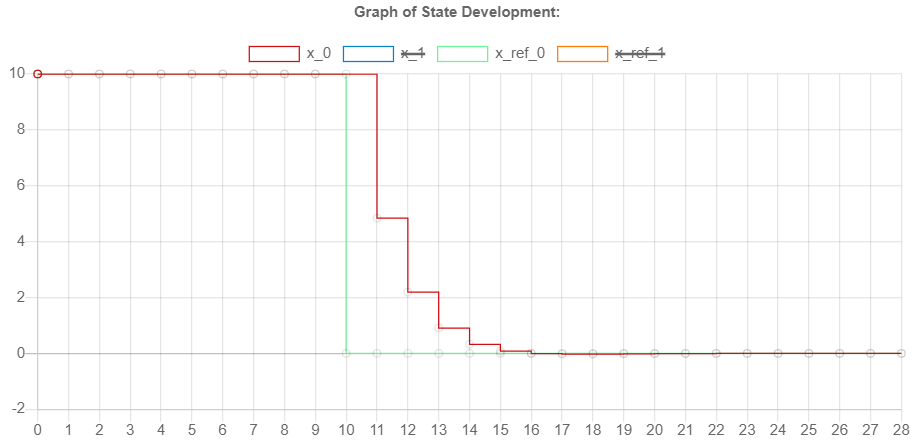
\includegraphics[width=13cm,height=7cm]{images/Hmotny_bod_apk/x0}
	\caption{Priebeh riadenia pre prvý stav systému}
\end{figure}
\begin{figure}[H]
	\centering
	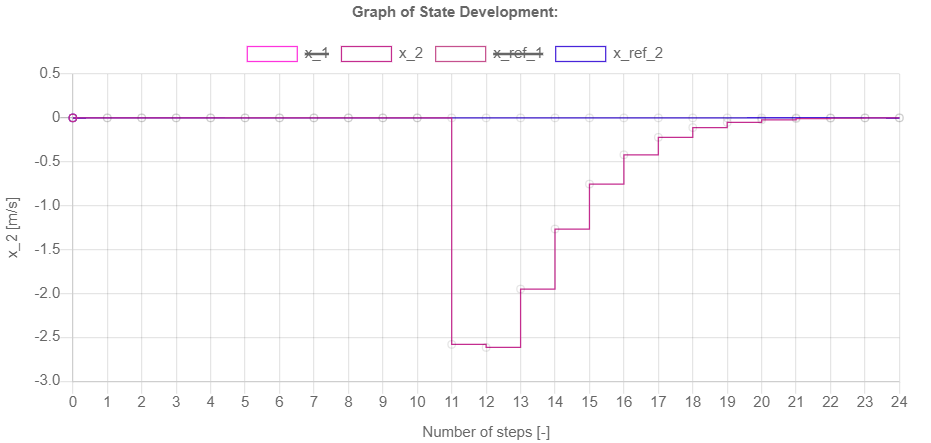
\includegraphics[width=13cm,height=7cm]{images/Hmotny_bod_apk/x1}
	\caption{Priebeh riadenia pre druhý stav systému}
\end{figure}
\begin{figure}[H]
	\centering
	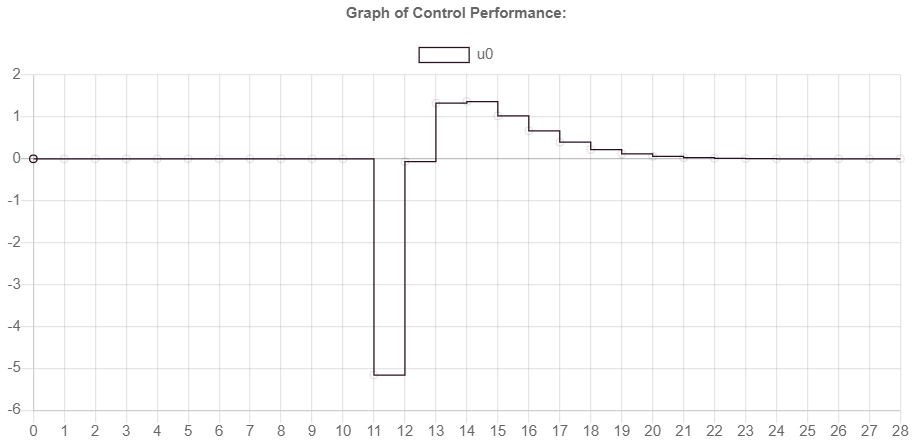
\includegraphics[width=13cm,height=7cm]{images/Hmotny_bod_apk/u}
	\caption{Vývoj akčných zásahov}
\end{figure}
Na grafoch (Obr. 4.8 až 4.10) môžeme vidieť priebeh simulácie. Pri porovnaní so simuláciou, ktorú sme vykonali v programovacom jazyku Matlab zistíme, že sú priebehy totožné, a preto považujeme našu aplikáciu za funkčnú. 

\chapter{Záver}
Cieľom tejto práce bolo navrhnúť, implementovať a overiť nový spôsob rýchleho riešenia optimalizačných problémov z oblasti prediktívneho riadenia. Metóda bola založená na rozdelení predikčného horizontu na menšie úseky s následným využitím distribuovaného optimalizačného algoritmu s možnosťou paralelného riešenia. Záver tejto práce sme venovali vývoju aplikácie, pomocou ktorej je možné využívať takýto spôsob riadenia s decentralizovaným MPC. 

V teoretickej časti sme si rozobrali formáciu predikatívneho regulátora založeného na lineárnom a nelineárnom modeli. Ďalej sme si vo všeobecnosti vysvetlili spôsob distribuovania optimalizačnej úlohy a jej následné riešenie pomocou ADMM, ktorá predstavovala algoritmus pre riešenie daného optimalizačného problému. V závere teórie sme si podrobne vysvetlili spôsob, akým využívame ADMM pri lineárnom a nelineárnom MPC. Pri lineárnom riadení sme použili analytickú optimalizáciu, kde sme položili gradient decentralizovanej účelovej funkcie (rozšírenej Lagrangianovej funkcie) rovný nule a vyjadrili sme si jednotlivé optimalizované premenné. Takýmto spôsobom sme získali všeobecné analytické vzorce, ktoré môžeme priamo využívať v ADMM. Pri komplikovanejšom nelineárnom riadení sme zvolili numerickú optimalizáciu, konkrétne Newtonovu metódu, ktorá slúži pre nájdenie minima decentralizovanej účelovej funkcie (rozšírenej Lagrangianovej funkcie). V tejto práci sme využívali aj ohraničenú optimalizáciu, ktorú sme ale pretransformovali do neohraničenej účelovej funkcie s logaritmickou bariérou.  

V praktickej časti sme si overili teóriu na diskrétnych simuláciách s cieľom zistiť, či takýmto spôsobom vieme zrýchliť výpočtový čas MPC. Simuláciu sme vykonali na dvoch systémoch s lineárnym a nelineárnym modelom. Lineárny model predstavoval zjednodušený pohyb hmotného bodu v priestore. Na základe simulácie sme prišli k záveru, že sa nám podarilo zrýchliť výpočtový čas linearného MPC. Nelineárny model reprezentoval skutočné zariadenie, konkrétne DC motor. Toto zariadenie je systém s veľmi rýchlou dynamikou $Ts = 50ms$. Preto nebolo cieľom dosiahnuť len lepší výpočtový čas ako pri centralizovanom nelineárnom MPC, ale museli sme ho znížiť natoľko, aby sa stíhal vypočítať akčný zásah v rámci periódy vzorkovania riadeného systému. To sa nám pomocou ladenia ADMM podarilo a značne sme zrýchlili výpočtový čas nelineárneho MPC. Môžeme prehlásiť, že takýto spôsob riadenia je možné využívať pre nelineárne systémy s rýchlou dynamikou. 

Ako posledné sme sa venovali vývoju aplikácie, pomocou ktorej vieme využívať decentralizované MPC s možnosťou paralelného riešenia na viacerých výpočtových zariadeniach. Vytvorili sme server v programovacom jazyku Python pomocou knižnice Flask. Server má viacero funkcií, slúži na prácu s dátami uloženými v databázach, vytvára distribuovaný optimalizačný problém z informácií od používateľa a prebieha na ňom diskrétna simulácia. Na strane klienta máme webové rozhranie. Pomocou tohoto rozhrania vie používateľ zadefinovať MPC a ovládať simuláciu. Má možnosť zastaviť simuláciu, alebo ju sledovať na dvoch grafoch v reálnom čase. Výsledky z jednotlivých numerických optimalizácií sú k dispozícií v dynamickej tabuľke. Táto optimalizácia prebieha na pozadí webového prehliadača v programovacom jazyku JavaScript (výpočtový klient). V závere sme vykonali experiment, ktorý potvrdil funkčnosť aplikácie a považujeme ju za správne navrhnutú podľa teórie. 

V budúcnosti by sa aplikácia dala vylepšiť tak, aby podporovala aj iný druh riadenia, ako je stavové MPC, alebo by bolo možné nahradiť simuláciu skutočným zariadením. 
% Appendices (Prílohy) comment by "%" if not neccesary
%\appendix
%\chapter{Resumé}
\label{ch:resume}

Resumé v slovenčine, sa píše v prípade, že záverečná práca ja napísaná v 
anglickom jazyku. Rozsah resumé tvorí 5-10\% rozsahu diplomovej práce.

%----------------------------------------------------------------%
%  The Backmatter !! Do NOT change the structure!!               %
%----------------------------------------------------------------%
% Bibliography to TOC
% do not remove
\backmatter
\providebibliography
\bibliography{bibfile}

%----------------------------------------------------------------%
%   The end of the document                                      %
%----------------------------------------------------------------%
\end{document}
